\chapter{结构}

\section{结构与同构}

本章的目的是一劳永逸地描述在数学中频繁出现的一定数量的构造性构造和证明（参见第一章，§1，第3节和§2，第2节）。

\subsection{层级（Echelons）}

一个层级构造方案是自然整数有序对的一个序列 \(c_1, c_2, \ldots, c_m\) （*） \(c_i = (a_i, b_i)\) ，满足以下条件：

\begin{enumerate}
\def\labelenumi{(\alph{enumi})}
\item
  如果 \(b_{i} = 0\) ，那么 \(1 \leqslant a_{i} \leqslant i - 1\) .
\item
  如果 \(a_i \neq 0\) 并且 \(b_i \neq 0\) ，那么 \(1 \leqslant a_i \leqslant i - 1\) 并且 \(1 \leqslant b_i \leqslant i - 1\) .
\end{enumerate}

这些条件蕴含 \(c_{1}=(0,b_{1})\) ，其中 \(b_{1}>0\) 。如果 n 是整数 \(b_{i}\) （它们出现在对 \((0,b_{i})\) 中）中最大的一个，那么 \(c_{1},c_{2},\ldots,c_{m}\) 则称其为 n 项上的层级构造方案。

给定一个 n 项上的层级构造方案 \(\mathbf{S} = (c_{1}, c_{2}, \ldots, c_{m})\) ，并给定理论 C 中的 n 个项 \(E_{1}, E_{2}, \ldots, E_{n}\) ，其中 C 是比集合论更强的理论，则方案 S 在 \(E_{1}, \ldots, E_{n}\) 上的一个层级构造被定义为理论 C 中的一个 m 项序列 \(A_{1}, A_{2}, \ldots, A_{m}\) ，由以下条件逐步定义：

\begin{enumerate}
\def\labelenumi{(\alph{enumi})}
\item
  如果 \(c_{i} = (0, b_{i})\) ，那么 \(A_{i}\) 是项 \(E_{b_{i}}\) .
\item
  如果 \(c_{i} = (a_{i}, 0)\) ，那么 \(A_{i}\) 是项 \(\mathfrak{P}(A_{a_i})\) .
\item
  如果 \(c_{i} = (a_{i}, b_{i})\) ，其中 \(a_{i} \neq 0\) 并且 \(b_{i} \neq 0\) ，那么 \(A_{i}\) 是项 \(A_{a_{i}} \times A_{b_{i}}\) .
\end{enumerate}

最后一项 \(A_{m}\) ，即方案 S 在 \(E_{1}, \ldots, E_{n}\) 上的阶梯构造的末项，称为方案 S 在基集合 \(E_{1}, \ldots, E_{n}\) 上的阶梯；在下文的一般论证中，它记作 \(S(E_{1}, \ldots, E_{n})\) .

示例。给定两个集合E，F，集合 \(\mathfrak{P}(\mathfrak{P}(E)) \times \mathfrak{P}(F)\) 是E，F上的一个阶梯，具有概形

\[
(0, 1), (0, 2), (1, 0), (3, 0), (2, 0), (4, 5).
\]

它也是E，F上的梯队，具有方案

\[
(0, 2), (0, 1), (1, 0), (2, 0), (4, 0), (5, 3).
\]

因此，不同的方案可能会在相同的条件下产生相同的梯队。

\subsection{映射的典范扩张}

设 \(S = (c_1, c_2, \ldots, c_m)\) 是一个具有 \(n\) 个项的阶梯构造方案。设 \(E_1, \ldots, E_n, E_1', \ldots, E_n'\) 为集合（即 \(\mathcal{G}\) 中的项），并设 \(f_1, \ldots, f_n\) 为 \(\mathcal{G}\) 中的项，使关系“ \(f_i\) 是从 \(E_i\) 到 \(E_i'\) 的映射”在 \(\mathcal{G}\) 中对每个 \(1 \leqslant i \leqslant n\) 都是定理。设 \(A_1, \ldots, A_m\) （分别地， \(A_1', \ldots, A_m'\) ) 为方案 S 在 \(E_1, \ldots, E_n\) （分别地， \(E_1', \ldots, E_n'\) ) 上的阶梯构造。我们按下述条件逐步定义一个由 \(m\) 个项 \(g_1, \ldots, g_m\) 组成的序列，使 \(g_i\) 是从 \(A_i\) 到 \(A_i'\) 的映射（ \(1 \leqslant i \leqslant m\) ）：

\begin{enumerate}
\def\labelenumi{(\alph{enumi})}
\item
  如果 \(c_{i} = (0, b_{i})\) ，因此 \(A_{i} = E_{b_{i}}\) 并且 \(A_{i}' = E_{b_{i}}'\) ，那么 \(g_{i}\) 是映射 \(f_{b_{i}}\) .
\item
  如果 \(c_{i} = (a_{i}, 0)\) ，因此 \(\mathbf{A}_{i} = \mathfrak{P}(\mathbf{A}_{a_{i}})\) 并且 \(\mathbf{A}_{i}' = \mathfrak{P}(\mathbf{A}_{a_{i}}')\) ，那么 \(g_{i}\) 是典范扩张 \(\hat{g}_{a_i}\) ，即 \(g_{a_i}\) 到子集族的扩张（第二章，第5节，第1号）。
\item
  如果 \(c_{i} = (a_{i}, b_{i})\) ，其中 \(a_{i} \neq 0\) 并且 \(b_{i} \neq 0\) ，因此
\end{enumerate}

\[
\mathrm{A} _ {i} = \mathrm{A} _ {a _ {i}} \times \mathrm{A} _ {b _ {i}} \quad \text { 且 } \quad \mathrm{A} _ {i} ^ {\prime} = \mathrm{A} _ {a _ {i}} ^ {\prime} \times \mathrm{A} _ {b _ {i}} ^ {\prime},
\]

则 \(g_{i}\) 是典范扩张 \(g_{a_i} \times g_{b_i}\) ，它将 \(g_{a_i}\) 和 \(g_{b_i}\) 扩张到 \(A_{a_i} \times A_{b_i}\) 上（第二章，第3节，第9号）。

该序列的最后一项 \(g_{m}\) 称为映射 \(f_{1}, \ldots, f_{n}\) 的具有方案S的典范扩张，并将用 \(\langle f_{1}, \ldots, f_{n} \rangle^{S}\) 表示。以下准则可以逐步验证：

CST1. 如果 \(f_{i}\) 是从 \(\mathbf{E}_i\) 到 \(\mathbf{E}_i'\) 的映射，并且如果 \(f_{i}'\) 是从 \(\mathbf{E}_i'\) 到 \(\mathbf{E}_i''\) 的映射 ( \(1 \leqslant i \leqslant n\) )，那么对于每个 \(n\) 项上的层级构造方案，我们有

\[
\langle f _ {1} ^ {\prime} \circ f _ {1}, f _ {2} ^ {\prime} \circ f _ {2}, \dots , f _ {n} ^ {\prime} \circ f _ {n} \rangle^ {\mathrm{S}} = \langle f _ {1} ^ {\prime}, f _ {2} ^ {\prime}, \dots , f _ {n} ^ {\prime} \rangle^ {\mathrm{S}} \circ \langle f _ {1}, f _ {2}, \dots , f _ {n} \rangle^ {\mathrm{S}}.
\]

CST2. 若 \(f_{i}\) 对 \(1 \leqslant i \leqslant n\) 是单射（相应地，满射），那么 \(\langle f_{1}, \ldots, f_{n} \rangle^{S}\) 是单射（相应地，满射）。

该判据由扩展的相应性质得出。 \(\hat{g}\) (第二章，§5，第1号，命题1)及扩展 \(g \times h\) （第二章，第3节，第9号）。

CST3. 如果 \(f_{i}\) 是 \(\mathbf{E}_i\) 到 \(\mathbf{E}_i'\) 上的双射，并且如果 \(f_{i}^{-1}\) 是(*)的逆双射，则 \(\langle f_1, \ldots, f_n \rangle^{S}\) 是一个双射且 \(\langle f_1^{-1}, \ldots, f_n^{-1} \rangle^{S}\) 是其逆；换言之，

\[
(\langle f _ {1}, \dots , f _ {n} \rangle^ {\mathrm{S}}) ^ {- 1} = \langle f _ {1} ^ {- 1}, \dots , f _ {n} ^ {- 1} \rangle^ {\mathrm{S}}.
\]

这直接从CST1和CST2得出。

\subsection{可迁移关系}

让 \(\mathfrak{C}\) 是一个比集合论更强的理论，设 \(x_{1},\ldots ,x_{n},\) \(s_1,\ldots ,s_p\) 是互不相同的字母，且与 \(\mathfrak{C}\) 的常元不同，并且设 \(\mathrm{A}_1,\ldots ,\mathrm{A}_m\) 为 \(\mathfrak{C}\) 中的项，其中字母 \(x_{i}\) \((1\leqslant i\leqslant n)\) 与 \(s_j\) \((1\leqslant j\leqslant p)\) 均不出现。设 \(\mathrm{S}_1,\ldots ,\mathrm{S}_p\) 是 \(n + m\) 项上的阶梯构造方案。则关系 \(\mathrm{T}\{x_1,\dots,x_n,s_1,\dots,s_p\}\) :

\[
\begin{array}{c}
\text{``}s_{1} \in S_{1}(x_{1}, \ldots, x_{n}, A_{1}, \ldots, A_{m})
\text{ 且 }s_{2} \in S_{2}(x_{1}, \ldots, x_{n}, A_{1}, \ldots, A_{m}) \\
\text{且 }\ldots\text{ 且 }s_{p} \in S_{p}(x_{1}, \ldots, x_{n}, A_{1}, \ldots, A_{m})\text{''}
\end{array}
\]

被称为字母的典型化 \(s_{1}, \ldots, s_{p}\) .

设 \(\mathbb{R}\{x_1, \ldots, x_n, s_1, \ldots, s_p\}\) 是 \(\mathfrak{C}\) 中的一个关系，其中含有某些字母 \(x_i, s_j\) （也可能含有其他字母）。如果满足下述条件，则称 \(\mathbb{R}\) 在 \(\mathfrak{C}\) 中对类型化 \(\mathbb{T}\) 是可迁移的，其中 \(x_i (1 \leqslant i \leqslant n)\) 视为主基集， \(A_h (1 \leqslant h \leqslant m)\) 视为辅助基集：设 \(y_1, \ldots, y_n, f_1, \ldots, f_n\) 是两两不同的字母，并且不同于 \(x_i (1 \leqslant i \leqslant n)\) 、 \(s_j (1 \leqslant j \leqslant p)\) 、 \(\mathfrak{C}\) 的常量，以及 \(\mathbb{R}\) 或各项 \(A_h (1 \leqslant h \leqslant m)\) 中出现的所有字母；再设 \(\operatorname{Id}_h (1 \leqslant h \leqslant m)\) 表示 \(A_h\) 到自身的恒等映射。则关系

\begin{enumerate}
\def\labelenumi{(\arabic{enumi})}
\tightlist
\item
  “T \(\{x_{1},\ldots,x_{n},s_{1},\ldots,s_{p}\}\) 且 ( \(f_{1}\) 是 \(x_{1}\) 到 \(y_{1}\) 上的双射 ) 且 \ldots{} 且 ( \(f_{n}\) 是 \(x_{n}\) 到 \(y_{n}\) 上的双射 )''
\end{enumerate}

蕴含，在 \(\mathfrak{G}\) ，关系

\[
\mathrm{R} \left\{x _ {1}, \dots , x _ {n}, s _ {1}, \dots , s _ {p} \right\} \Longleftrightarrow \mathrm{R} \left\{y _ {1}, \dots , y _ {n}, s _ {1} ^ {\prime}, \dots , s _ {p} ^ {\prime} \right\},\tag{2}
\]

其中

\[
s _ {j} ^ {\prime} = \left\langle f _ {1}, \dots , f _ {n}, \operatorname{Id} _ {1}, \dots , \operatorname{Id} _ {m} \right\rangle^ {S_j} (s _ {j}) \quad (1 \leqslant j \leqslant p).\tag{3}
\]

在没有辅助集合的情况下，存在一个类似但更简单的定义。

例如，如果 \(n = p = 2\) 并且如果类型化 \(\mathbf{T}\) 是“\(s_1 \in x_1\) 并且 \(s_2 \in x_1\)''，关系 \(s_1 = s_2\) 是可迁移的。另一方面，关系 \(x_1 = x_2\) 不是可迁移的。

\subsection{结构的种类}

让 \(\mathfrak{G}\) 是一个比集合论更强的理论。在 \(\mathfrak{G}\) 中的结构种类是一个文本 \(\Sigma\) 由以下汇编组成：

\begin{enumerate}
\def\labelenumi{(\arabic{enumi})}
\item
  一定数量的字母 \(x_1, \ldots, x_n, s\) ，彼此不同，且与常数 \(\mathfrak{G}\) ; \(x_1, \ldots, x_n\) 被称为该结构物种的主基集 \(\Sigma\) ;
\item
  一定数量的项 \(A_{1}, \ldots, A_{m}\) 在 G 中，其中没有一个字母 \(x_{1}, \ldots, x_{n}, s\) 出现，并且被称为辅助基集 \(\Sigma\) ; \(\Sigma\) 可能不包含任何辅助基集（但必须至少包含一个主基集）；
\item
  一种典型化 \(\mathrm{T}\{x_1, \ldots, x_n, s\}\) :
\end{enumerate}

\[
s \in \mathrm{S} (x _ {1}, \dots , x _ {n}, \mathrm{A} _ {1}, \dots , \mathrm{A} _ {m}),
\]

其中 S 是定义在 \(n + m\) 术语（编号1）；T \(\{x_{1}, \ldots, x_{n}, s\}\) 被称为结构种类的典型刻画 \(\Sigma\) ;

\begin{enumerate}
\def\labelenumi{(\arabic{enumi})}
\setcounter{enumi}{3}
\tightlist
\item
  一个关系 \(R\{x_{1},\ldots,x_{n},s\}\) 该关系在类型化T下（在C中）是可迁移的， \(x_{i}\) 作为主基集和 \(A_{h}\) 辅助基集（第3号）；R被称为结构种类的公理 \(\Sigma\) .
\end{enumerate}

理论 \(C_{\Sigma}\) 具有与C相同的公理模式，其显式公理为C的公理，再加上公理“T和R”，称为结构物种的理论 \(\Sigma\) 。 \(C_{\Sigma}\) 的常量因此是C的常量以及出现在T或R中的字母。

让 \(\mathfrak{C}'\) 是比 \(\mathfrak{C}\) 更强的理论，并且让 \(\mathbf{E}_1, \ldots, \mathbf{E}_n\) ，U是 \(\mathfrak{C}'\) 中的项。在理论 \(\mathfrak{C}'\) 中，U被称为物种 \(\Sigma\) 在主基集上 \(\mathbf{E}_1, \ldots, \mathbf{E}_n\) ，以 \(\mathbf{A}_1, \ldots, \mathbf{A}_m\) 作为辅助基集，如果该关系

\[
" \mathrm{T} \left\{\mathrm{E} _ {1}, \dots , \mathrm{E} _ {n}, \mathrm{U} \right\} \text { 且 } \mathrm{R} \left\{\mathrm{E} _ {1}, \dots , \mathrm{E} _ {n}, \mathrm{U} \right\}"
\]

在 \(\mathfrak{C}'\) 中是定理。当这种情况发生时，对于每个定理 \(\mathbf{B}\{x_1, \ldots, x_n, s\}\) （在理论 \(\mathfrak{C}_{\Sigma}\) 中），关系 \(\mathbf{B}\{\mathrm{E}_1, \ldots, \mathrm{E}_n, \mathrm{U}\}\) 在 \(\mathfrak{C}'\) 中是定理（第一章，§2，第3号）。在 \(\mathfrak{C}_{\Sigma}\) 中，常量 \(s\) 被称为物种 \(\Sigma\) .

的泛型结构。在理论 \(\mathfrak{G}'\) 中，主基集 \(\mathbf{E}_1, \ldots, \mathbf{E}_n\) 被称为具有结构U。显然，U是集合

\[
\mathrm{S} (\mathbf {E} _ {1}, \dots , \mathbf {E} _ {n}, \mathbf {A} _ {1}, \dots , \mathbf {A} _ {m}).
\]

因此， \(\mathrm{S}(\mathbf{E}_{1},\ldots,\mathbf{E}_{n},\mathbf{A}_{1},\ldots,\mathbf{A}_{m})\) 中满足关系 \(R\{\mathbf{E}_{1},\ldots,\mathbf{E}_{n},\mathbf{V}\}\) 的元素 V 所成的集合，就是种类 \(\Sigma\) 在基集 \(E_{1},\ldots,E_{n}\) 上的所有结构之集（它可能是空集）。

示例

\begin{enumerate}
\def\labelenumi{(\arabic{enumi})}
\tightlist
\item
  取 \(\mathfrak{C}\) 为集合论，并考虑这样一种结构：它没有辅助基集，只有一个主基集 A，典型特征为 \(s \in \mathfrak{P}(A \times A)\) ，公理为
\end{enumerate}

\[
s \circ s = s \quad \text { 且 } \quad s \cap \overline{s} = \Delta_{\mathbf{A}}
\]

\((\Delta_{\mathbf{A}}\) 为对角线 \(\mathbf{A} \times \mathbf{A})\) ，这是关于类型化的一种可迁移关系 \(s \in \mathfrak{P}(\mathbf{A} \times \mathbf{A})\) ，这一点很容易验证。显然，这类结构的理论正是有序集的理论（第三章，§1，第3节）；因此，这样定义的结构类型也被称为 \(\mathbf{A}\) 上的序结构物种。在第三章中，我们看到了许多带有这种物种结构的集合的例子。

\begin{enumerate}
\def\labelenumi{(\arabic{enumi})}
\setcounter{enumi}{1}
\item
  取 \(\mathfrak{G}\) 为集合论，并考虑这样一种结构：它没有辅助基集，只有一个主基集 A，典型特征为 \(F \in \mathfrak{P}((A \times A) \times A)\) ，公理是可迁移关系“F 是一个定义域为 \(A \times A\) 的函数图”。这种结构是所谓代数结构的特例；以 F 为图的函数（从 \(A \times A\) 到 A 的映射），称为这种结构的（处处有定义的）内部合成律。
\item
  和之前一样，令 \(\mathfrak{C}\) 设集合论为理论，并考虑这样的结构类，它没有辅助基集，只有一个主基集A，其典型特征为 \(V \in \mathfrak{P}(\mathfrak{P}(A))\) ，以及作为公理的可迁移关系
\end{enumerate}

\[
\begin{array}{l} (\forall \mathrm{V}) ((\mathrm{V} ^ {\prime} \subset \mathrm{V}) \Longrightarrow ((\bigcup_ {\mathrm{X} \in \mathrm{V} ^ {\prime}} \mathrm{X}) \in \mathrm{V})) \\ \text { 且 } \quad (\forall \mathrm{X}) (\forall \mathrm{Y}) ((\mathrm{X} \in \mathrm{V} \text {   且   } \mathrm{Y} \in \mathrm{V}) \Longrightarrow ((\mathrm{X} \cap \mathrm{Y}) \in \mathrm{V})). \end{array}
\]

这种结构类型被称为拓扑结构类型。这种类型的一个结构也称为拓扑，而该关系 \(X \in V\) 用拓扑V中的开集X来表示（一般拓扑学，第一章，§1）。

* (4) 取 \(\mathfrak{G}\) 作为除环结构这个物种的理论，其（除其他事项外）有一个常数K作为唯一的（主）基集。K上的左向量空间这一结构物种以K为辅助基集，以E为主基集，其典型特征关系为

\[
\mathbf {V} \in \mathfrak {P} ((\mathbf {E} \times \mathbf {E}) \times \mathbf {E}) \times \mathfrak {P} ((\mathbf {K} \times \mathbf {E}) \times \mathbf {E})
\]

\((pr_{1}V \text{ 是 } E \text{ 中加法的图，而 } pr_{2}V \text{ 是标量乘法的图 }); \text{ 我们在此不陈述该结构物种的公理。}\)

\begin{enumerate}
\def\labelenumi{(\arabic{enumi})}
\setcounter{enumi}{4}
\tightlist
\item
  再次令 \(\mathfrak{G}\) 是集合论；在这个理论中，复数域 \(\mathbf{C}\) 是一个不含字母的项。维数为 \(n\) 的复解析流形的结构种具有 \(\mathbf{C}\) 作为辅助基集，以及一个主基集 \(V\) 我们在此不指出这类结构的典型特征或公理。*
\end{enumerate}

\minorheading{注记}

\begin{enumerate}
\def\labelenumi{(\arabic{enumi})}
\tightlist
\item
  在应用中，常常出现（如上述例4中）梯队 \(S(E_1, \ldots, E_n, A_1, \ldots, A_m)\) 是若干梯队的乘积。
\end{enumerate}

\[
\mathrm{S} _ {1} \left(\mathrm{E} _ {1}, \dots , \mathrm{A} _ {m}\right) \times \dots \times \mathrm{S} _ {p} \left(\mathrm{E} _ {1}, \dots , \mathrm{A} _ {m}\right).
\]

若是如此，在 \(s\) 的定义中，字母 \(\Sigma\) 常被替换为一个“ \(p\) 元组” \((s_{1}, \ldots, s_{p})\) （参见第二章，第2节，第1号）。

此外，结构种类的公理 \(\Sigma\) 通常被写成若干可迁移关系的合取（如上面的例3所示）。这些关系被称为该物种的公理。 \(\Sigma\) .

\begin{enumerate}
\def\labelenumi{(\arabic{enumi})}
\setcounter{enumi}{1}
\item
  数学中最常用的结构种类，以及赋予这些结构种类的集合，都有特定的名称。因此，有序集（第三章，§1）是赋予序结构（例1）的集合；* 在本系列后续的卷册中，我们将定义群、域、拓扑空间、微分流形等概念，所有这些都指代赋予特定结构的集合。*
\item
  按照惯例，在集合论中 \(\mathfrak{G}\) ，赋予 \(n\) 不同的字母 \(x_{1},\ldots,x_{n}\) （没有典型刻画且没有公理）被视为结构的一种 \(\Sigma_{0}\) ，称为集合上的结构， \(n\) 主基集 \(x_{1},\ldots,x_{n}\) .
\end{enumerate}

\subsection{同构与结构的迁移}

让 \(\Sigma\) 是理论中的一类结构 \(\mathfrak{C}\) ，在 \(n\) 主基集 \(x_{1},\ldots ,x_{n}\) ，以 \(m\) 辅助基集 \(\mathbf{A}_1,\dots ,\mathbf{A}_m\) . 设 \(\mathbf{S}\) 设为关于 \(n + m\) 字母的阶梯构造方案，该方案出现在以下典型刻画中 \(\Sigma\) ，并且让 \(\mathbf{R}\) 是……的公理 \(\Sigma\) 。在一个理论中 \(\mathfrak{C}'\) 该理论强于 \(\mathfrak{C}\) ，让 \(\mathbf{U}\) 是物种的一个结构 \(\Sigma\) 关于集合 \(\mathbf{E}_1,\ldots ,\mathbf{E}_n\) （作为主基集）并令 \(\mathbf{U}'\) 是集合上同一种类的结构 \(\mathbf{E}_1',\ldots ,\mathbf{E}_n'\) 。最后，令 \(f_{i}\) （在 \(\mathfrak{C}'\) ）是 \(\mathbf{E}_i\) 到 \(\mathbf{E}_i'\) 上的双射 ( \(1 \leqslant i \leqslant n\) )。然后 \((f_1, \ldots, f_n)\) 被称为这些集合之间的同构 \(\mathbf{E}_1, \ldots, \mathbf{E}_n\) ，赋予该结构 \(\mathbf{U}\) 到集合 \(\mathbf{E}_1', \ldots, \mathbf{E}_n'\) ，赋予该结构 \(\mathbf{U}'\) ，如果我们有（在 \(\mathfrak{C}'\) )

\[
\langle f _ {1}, \dots , f _ {n}, \operatorname{Id} _ {1}, \dots , \operatorname{Id} _ {m} \rangle^ {\mathrm{s}} (\mathrm{U}) = \mathrm{U} ^ {\prime}\tag{4}
\]

其中 \(Id_{h}\) 表示 \(A_{h}\) 到自身的恒等映射（ \(1 \leqslant h \leqslant m\) ）。¶ 设 \(f_{i}^{\prime}\) 是双射 \(f_{i}\) 的逆映射（ \(1 \leqslant i \leqslant n\) ）。由（4）和准则 CST3（第2号）立即得到

\[
\langle f _ {1} ^ {\prime}, \dots , f _ {n} ^ {\prime}, \operatorname{Id} _ {1}, \dots , \operatorname{Id} _ {m} \rangle^ {\mathrm{s}} (\mathbf {U} ^ {\prime}) = \mathbf {U}
\]

，因此 \((f_1', \ldots, f_n')\) 是……的一个同构 \(\mathbf{E}_1', \ldots, \mathbf{E}_n'\) ，赋予 \(\mathbf{U}'\) ，映到 \(\mathbf{E}_1, \ldots, \mathbf{E}_n\) ，赋予 \(\mathbf{U}\) 。这些同构 \((f_1, \ldots, f_n)\) 并且 \((f_1', \ldots, f_n')\) 被称为彼此的逆。

\(E_{1}^{\prime}, \ldots, E_{n}^{\prime}\) ，赋予 \(U^{\prime}\) ，若存在 \(E_{1}, \ldots, E_{n}\) 的一个同构，则称其与 \(E_{1}, \ldots, E_{n}\) 到上 \(E_{1}^{\prime}, \ldots, E_{n}^{\prime}\) （赋予U）同构；在这种情况下，结构U与 \(U^{\prime}\) 被称为同构的。上述定义，连同CST1，蕴含以下判据：

CST4. 设 U， \(U'\) , \(U''\) 是同一物种的三个结构 \(\Sigma\) 在主基集上 \(E_{1}, \ldots, E_{n}, E_{1}', \ldots, E_{n}', E_{1}'', \ldots, E_{n}''\) 是物种 \(f_{i}\) 是……的双射 \(E_{i}\) 到上 \(E_{i}'\) ，并且让 \(g_{i}\) 是……的双射 \(E_{i}'\) 到上 \(E_{i}''\) ( \(1 \leqslant i \leqslant n\) ）。如果 \((f_{1}, \ldots, f_{n})\) 并且 \((g_{1}, \ldots, g_{n})\) 都是同构，则 \((g_{1} \circ f_{1}, \ldots, g_{n} \circ f_{n})\) .

的一个同构 \(E_{1}, \ldots, E_{n}\) 到上 \(E_{1}, \ldots, E_{n}\) （关于同一结构）称为 \(E_{1}, \ldots, E_{n}\) 的自同构。 \(E_{1}, \ldots, E_{n}\) 的两个自同构的复合仍是自同构，自同构的逆也是自同构，* 因此 \(E_{1}, \ldots, E_{n}\) 的自同构构成一个群。*

注记。按照语言的滥用，如果 \(f_{i}\) 是...的任意双射 \(\mathbf{E}_i\) 到上 \(\mathbf{E}_i'\) ( \(1 \leqslant i \leqslant n\) ), \((f_1, \ldots, f_n)\) 被称为...的一个同构 \(\mathbf{E}_1, \ldots, \mathbf{E}_n\) 到上 \(\mathbf{E}_1', \ldots, \mathbf{E}_n'\) 关于集合的结构种（第4号，注记3）。

CST5. 在一个理论 \(\mathfrak{G}'\) 该理论强于 \(\mathfrak{G}\) 中，设U是物种 \(\Sigma\) 在 \(\mathbf{E}_1, \ldots, \mathbf{E}_n\) 上的一个结构，并且让 \(f_i\) 是……的双射 \(\mathbf{E}_i\) 到集合 \(\mathbf{E}_i'\) ( \(1 \leqslant i \leqslant n\) ). 那么存在唯一的物种 \(\Sigma\) 在 \(\mathbf{E}_1', \ldots, \mathbf{E}_n'\) 上的结构，使得 \((f_1, \ldots, f_n)\) 是……的一个同构 \(\mathbf{E}_1, \ldots, \mathbf{E}_n\) 到上 \(\mathbf{E}_1', \ldots, \mathbf{E}_n'\) .

对于这个结构，如果它存在，只能是项 \(U'\) 由关系(4)定义；仍需验证该项确实是物种 \(\Sigma\) 的结构，即关系 \(R\{E_{1}', \ldots, E_{n}', U'\}\) 在 \(C'\) . 但这由以下事实推出： \(R\{x_{1}, \ldots, x_{n}, s\}\) 是可迁移的，因为

\(R\{E_{1}^{\prime},\ldots,E_{n}^{\prime},U^{\prime}\}\) 在 \(C'\) 中等价于关系 \(R\{E_{1},\ldots,E_{n},U\}\) （第3号），而该关系在 \(C'\) 中由假设为真。

该结构 \(U'\) 被称为通过将结构U传输到集合而得到的 \(E_{1}^{\prime}, \ldots, E_{n}^{\prime}\) 通过双射映射 \(f_{1}, \ldots, f_{n}\) 因此，同一类型的两个结构是同构的，当且仅当每一个都是通过结构的迁移从另一个得到的。

可能发生这样的情况：任意两个类型为 \(\Sigma\) 的结构必然是同构的；结构类型 \(\Sigma\) 则称为单叶的。* 这就是无限循环群的结构（同构于 \(\mathbf{Z}\) ），特征为零的素域的结构（同构于 \(\mathbf{Q}\) ），完备阿基米德有序域的结构（同构于 \(\mathbf{R}\) ），一个代数闭的、连通的、局部紧致拓扑域的结构（同构于 \(\mathbf{C}\) ),以及非交换、连通、局部紧拓扑除环（同构于 \(\mathbf{H}\) ，即四元数除环）。对于其中某些结构类型，例如特征为零的素域，或完备的阿基米德有序域，甚至不存在除恒等映射以外的任何自同构；但对于上述给出的其他例子，确实存在这样的自同构（例如，对称 \(x \to -x\) 在 \(\mathbf{Z}\) ). *

可以观察到，上述结构种类本质上正是经典数学基础所依据的那些结构。另一方面，* 群结构的种类、有序集结构的种类以及拓扑结构的种类，并不是单价的。*

\subsection{结构的推导}

设 \(\Sigma\) 是理论 \(\mathfrak{G}\) 中的一种结构，它有 \(n\) 个主基集 \(x_{1},\ldots ,x_{n}\) 和 \(m\) 个辅助基集 \(\mathrm{A}_1,\dots ,\mathrm{A}_m\) . 设 \(s\) 是种类 \(\Sigma\) 的一般结构， \(\mathbf{T}\) 是一个具有 \(n + m\) 个项的阶梯构造方案。若项 \(\mathrm{V}\{x_1,\dots,x_n,s\}\) 除了所在理论的常量外不含其他字母（这里的理论为 \(\mathfrak{G}_{\Sigma}\) ），则在它满足下述条件时，称它对 \(s\) 是内在的，其类型为 \(\mathrm{T}(x_1,\dots,x_n,\mathrm{A}_1,\dots,\mathrm{A}_m)\) ：

\begin{enumerate}
\def\labelenumi{(\arabic{enumi})}
\item
  该关系 \(\mathbf{V}\{x_1, \ldots, x_n, s\} \in \mathbf{T}(x_1, \ldots, x_n, A_1, \ldots, A_m)\) 是定理于 \(\mathfrak{G}_{\Sigma}\) ;
\item
  让 \(\mathfrak{G}_{\Sigma}^{\prime}\) 为由以下公理添加到 \(\mathfrak{G}_{\Sigma}\) 的公理''所得到的理论 \(f_{i}\) 是 \(x_{i}\) 到上 \(y_{i}''\) ( \(1 \leqslant i \leqslant n\) ) 的双射（其中字母 \(y_{i}\) 并且 \(f_{i}\) 彼此不同，且不同于 \(\mathfrak{G}_{\Sigma}\) ，用于 \(1 \leqslant i \leqslant n\) 的常数；如果 \(s'\) 是通过 \(s\) 进行传输所得到的结构 \((f_{1}, \ldots, f_{n})\) （第5号），然后
\end{enumerate}

\[
\mathrm{V} \left\{y _ {1}, \dots , y _ {n}, s ^ {\prime} \right\} = \langle f _ {1}, \dots , f _ {n}, \operatorname{Id} _ {1}, \dots , \operatorname{Id} _ {m} \rangle^ {\mathrm{T}} (\mathrm{V} \left\{x _ {1}, \dots , x _ {n}, s \right\})
\]

是定理于 \(\mathfrak{C}_{\Sigma}^{\prime}\) .

在结构种类的理论中，人们被引导去定义的大多数术语都是内在术语。

让 \(\Theta\) 是理论中另一种结构种类 \(\mathfrak{G}\) ，在 \(r\) 主基集 \(u_{1},\ldots,u_{r}\) ，以 \(p\) 辅助基集 \(\mathrm{B}_{1},\ldots,\mathrm{B}_{p}\) ，并且让 \(t\in\mathrm{T}(u_{1},\ldots,u_{r},\mathrm{B}_{1},\ldots,\mathrm{B}_{p})\) 是……的典型刻画 \(\Theta\) （第4号）。那么，一个 \(r+1\) 项 \(\mathrm{P},\mathrm{U}_{1},\ldots,\mathrm{U}_{r}\) 的系统，对于 \(s\) ，并且使得 \(\mathrm{P}\) 是属于物种 \(\Theta\) 的、在 \(\mathrm{U}_{1},\ldots,\mathrm{U}_{r}\) 上的一个结构（在理论 \(\mathfrak{G}_{\Sigma}\) 中），被称为物种 \(\Theta\) 的结构由物种 \(\Sigma\) 的结构演绎而得的一个演绎程序。滥用语言时，术语 \(\mathrm{P}\) 单独常被称为演绎程序。

让 \(\mathfrak{G}'\) 为比……更强的理论 \(\mathfrak{G}\) 。如果 \(\mathcal{G}\) 是 \(\mathfrak{G}'\) 中物种 \(\Sigma\) 在 \(\mathrm{E}_1, \ldots, \mathrm{E}_n\) 上的一个结构，那么 \(\mathrm{P}\{\mathrm{E}_1, \ldots, \mathrm{E}_n, \mathcal{S}\}\) 是物种 \(\Theta\) 在这 \(r\) 个集合 \(\mathrm{F}_j = \mathrm{U}_j\{\mathrm{E}_1, \ldots, \mathrm{E}_n, \mathcal{S}\}(1 \leqslant j \leqslant r)\) 上的一个结构，称为由 \(\mathcal{S}\) 通过过程P，或从属于 \(\mathcal{G}\) 。假设项P， \(\mathrm{U}_1, \ldots, \mathrm{U}_r\) 对……是内在的 \(s\) 此外还蕴含以下判据：

CST6。 让 \((g_{1}, \ldots, g_{n})\) 是……的一个同构 \(E_{1}, \ldots, E_{n}\) ，配备有物种 \(\Sigma\) ，映到 \(E_{1}^{\prime}, \ldots, E_{n}^{\prime}\) 的结构，配备有结构 \(S^{\prime}\) 同一物种的。如果 \(U_{j}\) 是类型 \(\mathfrak{P}(T_{j})\) 的严格递增映射，令

\[
h _ {j} = \left\langle g _ {1}, \dots , g _ {n}, \operatorname{Id} _ {1}, \dots , \operatorname{Id} _ {m} \right\rangle^ {\mathrm{T}_j} \quad (1 \leqslant j \leqslant r),
\]

并令 \(\mathbf{F}_j' = \mathbf{U}_j\{\mathbf{E}_1', \ldots, \mathbf{E}_n', \mathcal{S}'\} (1 \leqslant j \leqslant r)\) 。然后 \((h_1, \ldots, h_r)\) 是……的一个同构 \(\mathbf{F}_1, \ldots, \mathbf{F}_r\) 到上 \(\mathbf{F}_1', \ldots, \mathbf{F}_r'\) 当这些集合系统被赋予物种结构时 \(\Theta\) 由...推导出 \(\mathcal{S}\) 并且 \(\mathcal{S}'\) 分别通过过程P。

显然，项 \(x_{1}, \ldots, x_{n}\) 对……是内在的 \(s\) 在许多情况下，项 \(U_{1}, \ldots, U_{r}\) 是某些字母 \(x_{1}, \ldots, x_{n}\) ；物种的结构 \(\Theta\) 由...推导出 \(s\) 通过该程序 \(P\) 随后被称为底层结构 \(s\) .

\minorheading{示例}

* (1) 拓扑群结构的物种具有一个主基集A，没有辅助基集，相应的典型结构是一个对 \((s_1, s_2)\) ( \(s_1\) 是A上合成律的图，而 \(s_2\) 是A拓扑中的开集族；参见《一般拓扑学》第三章第1节）。每一项 \(s_1\) , \(s_2\) 都是一个推导过程，分别提供拓扑群结构所依据的群结构和拓扑。 \((s_1, s_2)\) .

同样地，从向量空间结构可以推导出底层的交换群结构。从环结构可以推导出底层的交换群结构和（乘法）半群结构。从可微流形结构可以推导出底层的拓扑，等等。

\begin{enumerate}
\def\labelenumi{(\arabic{enumi})}
\setcounter{enumi}{1}
\tightlist
\item
  复数域C（相应地，实数域R）上向量空间结构的物种具有一个主基集E，一个等于C（相应地，R）的辅助基集，以及典型刻画
\end{enumerate}

\[
s _ {1} \in \mathfrak {P} ((\mathbf {E} \times \mathbf {E}) \times \mathbf {E}) \quad \text { 且 } \quad s _ {2} \in \mathfrak {P} ((\mathbf {C} \times \mathbf {E}) \times \mathbf {E})
\]

\[
(\text { 分别 } \quad s _ {1} \in \mathfrak {P} ((E \times E) \times E) \quad \text { 且 } \quad s _ {2} \in \mathfrak {P} ((R \times E) \times E)).
\]

对 \((s_{1}, s_{2} \cap ((\mathbf{R} \times \mathbf{E}) \times \mathbf{E}))\) 是从复数域C上的向量空间结构推导实数域R上的向量空间结构的过程（“将标量域限制为R”）。*

\begin{enumerate}
\def\labelenumi{(\arabic{enumi})}
\setcounter{enumi}{2}
\tightlist
\item
  假设 \(\Theta\) 具有与 \(\Sigma\) 相同的主基集和辅助基集，以及相同的典型刻画。此外，如果 \(\Sigma\) 的公理蕴含（在 \(\mathfrak{C}\) ) 公理 \(\Theta\) ，显然该项 \(s\) 是从物种结构 \(\Theta\) 到物种结构的演绎程序 \(\Sigma\) . \(\Theta\) 则被称为比……更贫乏 \(\Sigma\) ，以及 \(\Sigma\) 比……更丰富 \(\Theta\) 。每个属于物种 \(\Sigma\) 的结构，在理论 \(\mathfrak{C}'\) 该理论强于 \(\mathfrak{C}\) ，则也是物种 \(\Theta\) 的一个结构。例如，全序集结构的物种（通过取序结构公理（第4节，例1）与关系
\end{enumerate}

的合取作为公理而得到）比序结构的物种更丰富。*交换群结构的物种比群结构的物种更丰富。紧致拓扑空间结构的物种比拓扑结构的物种更丰富，等等。* \(s \cup \overline{s} = A \times A\) *（4）当

各自是群结构（相应地，环结构）的物种时，在代数中定义了一种演绎程序，它将每个群结构（相应地，环结构）与其中心上的群结构（相应地，环结构）相关联。当 \(\Sigma\) 并且 \(\Theta\) 是域K上向量空间结构的物种，且 \(\Sigma\) 是K上代数结构的物种时，定义了演绎程序，将K上的每个向量空间与其张量代数或外代数相关联。在本系列的后续部分，我们还会遇到许多其他例子。* \(\Theta\) 7. 等价的结构物种

注记。当P是一个“q元组”时 \((P_{1}, \ldots, P_{q})\) ，也称这些项 \(P_{1}, \ldots, P_{q}\) 构成一个物种结构的演绎过程 \(\Theta\) 到物种结构的演绎程序 \(\Sigma\) .

\subsection{是同一理论}

让 \(\Sigma\) 并且 \(\Theta\) 中的两个结构物种，具有相同的主基集 \(\mathfrak{C}\) 分别是物种 \(x_{1},\ldots ,x_{n}\) . 设 \(s,t\) 的泛结构。假设满足以下条件： \(\Sigma,\Theta\) 关系

\begin{enumerate}
\def\labelenumi{(\arabic{enumi})}
\item
  我们有一个演绎过程 \(\mathbf{P}\{x_1, \ldots, x_n, s\}\) ，把物种 \(\Theta\) 在 \(x_1, \ldots, x_n\) 上的结构由物种 \(\Sigma\) 在 \(x_1, \ldots, x_n\) 上的结构演绎出来。
\item
  我们有一个演绎过程 \(\mathbb{Q}\{x_1, \ldots, x_n, t\}\) ，把物种 \(\Sigma\) 在 \(x_1, \ldots, x_n\) 上的结构由物种 \(\Theta\) 在 \(x_1, \ldots, x_n\) 上的结构演绎出来。
\item
  ，以及关系 \(\mathbf{Q}\{x_1, \ldots, x_n, \mathbf{P}\{x_1, \ldots, x_n, s\}\} = s\) 是定理于 \(\mathfrak{G}_{\Sigma}\) ，关系B \(\mathbf{P}\{x_1, \ldots, x_n, \mathbf{Q}\{x_1, \ldots, x_n, t\}\} = t\) 是定理于 \(\mathfrak{G}_{\Theta}\) .
\end{enumerate}

结构的物种 \(\Sigma\) 并且 \(\Theta\) 则称通过演绎程序P和Q是等价的。在这种情况下，对于每一个定理B \(\{x_1, \ldots, x_n, s\}\) 在该理论中 \(\mathfrak{G}_{\Sigma}\) ；反之，对于每个定理C \(\{x_1, \ldots, x_n, Q\}\) 是定理于 \(\mathfrak{G}_{\Theta}\) ，关系C \(\{x_1, \ldots, x_n, t\}\) 在该理论中 \(\mathfrak{G}_{\Theta}\) 如果U是物种 \(\{x_1, \ldots, x_n, P\}\) 是定理于 \(\mathfrak{G}_{\Sigma}\) .

的一个结构，则由程序P从U演绎出的结构称为与U等价。准则CST6蕴含以下结论： \(\Sigma\) CST7. 设

分别是物种 \(\mathcal{S},\mathcal{S}'\) 的两个结构。设 \(\Sigma\) 在主基集上 \((\mathbf{E}_1,\ldots ,\mathbf{E}_n),(\mathbf{E}_1',\ldots ,\mathbf{E}_n')\) 是物种 \(\mathcal{S}_0,\mathcal{S}_0'\) 的结构，它们分别与 \(\Theta\) 等价。 \(\mathcal{S}\) 并且 \(\mathcal{S}'\) 。为了使得 \((g_1,\dots,g_n)\) 是关于结构 \(\mathcal{S}_0\) 并且 \(\mathcal{S}_0'\) 的一个同构，当且仅当 \((g_1,\dots,g_n)\) 是关于结构 \(\mathcal{S}\) 并且 \(\mathcal{S}'\) .

在实践中，我们不区分两个等价结构物种的理论 \(\mathfrak{G}_{\Sigma}\) 并且 \(\mathfrak{G}_{\Theta}\) 。

\minorheading{示例}

*（1）设 \(\Sigma\) 是交换群结构的物种； \(\Sigma\) 有一个（主）基集A，其泛结构由单个字母F组成； \(\Sigma\) 是 \(F \in \mathfrak{P}((A \times A) \times A)\) 的典型刻画，并且我们将 \(\Sigma\) 的公理记为R \{A, F\}。该公理特别蕴含F是某个函数的图（群的“合成律”；参见第4节，例2）。在理论 \(\mathfrak{G}_{\Sigma}\) （其中 \(\mathfrak{G}\) 表示集合论）中，我们定义一个项M\{A, F\} ，它是 \(\mathfrak{P}((Z \times A) \times A)\) 中的一个函数图，并满足以下关系B\{M, A, F\}:

\((\forall x)(\forall y)(\forall n)((x \in A \text{ 且 } y \in A \text{ 且 } n \in \mathbf{Z})\)

\[
\Longrightarrow (\mathbf {M} (n, \mathrm{F} (x, y)) = \mathrm{F} (\mathbf {M} (n, x), \mathrm{M} (n, y))))
\]

并且 \((\forall x)(\forall m)(\forall n)((x\in A\) 并且 \(m\in \mathbf{Z}\) 并且 \(n\in \mathbf{Z})\)

\[
\Rightarrow (\mathrm{M} (m + n, x) = \mathrm{F} (\mathrm{M} (m, x), \mathrm{M} (n, x))))
\]

并且 \((\forall x)(\forall m)(\forall n)((x\in A\) 并且 \(m\in \mathbf{Z}\) 并且 \(n\in \mathbf{Z})\)

\[
\Longrightarrow (\mathbf {M} (m, \mathbf {M} (n, x)) = \mathbf {M} (m n, x)))
\]

并且

\[
(\forall x) ((x \in A) \Longrightarrow (M (1, x) = x)).
\]

（“A 的元素与整数相乘”）。

考虑该物种 \(\Theta\) 的 \(\mathbf{Z}\) -模结构，其具有单一的主基集 A，其中 \(\mathbf{Z}\) 作为辅助集合，其一般结构包含两个字母G、L，具有典型的刻画

\[
\mathbf {G} \in \mathfrak {P} ((\mathbf {A} \times \mathbf {A}) \times \mathbf {A}) \quad \text { 且 } \quad \mathbf {L} \in \mathfrak {P} ((\mathbf {Z} \times \mathbf {A}) \times \mathbf {A})
\]

以及公理

\[
\text{``}R\{A,G\}\text{ 且 }(L\text{ 是函数图})\text{ 且 }B\{L,A,G\}\text{''.}
\]

立即验证可知，项F、M构成了一种物种结构的演绎程序。 \(\Theta\) 到物种结构的演绎程序 \(\Sigma\) ，并且项 G 是物种结构的一个演绎过程 \(\Sigma\) 到物种结构的演绎程序 \(\Theta\) 。此外，上述条件（3）平凡地成立。因此我们可以说，交换群结构的物种与 Z-模结构的物种是等价的。

\begin{enumerate}
\def\labelenumi{(\arabic{enumi})}
\setcounter{enumi}{1}
\tightlist
\item
  让 \(\Sigma\) 是拓扑结构的种类（第4号，例3），设A为（主）基集，并设V为 \(\Sigma\) 。考虑关系
\end{enumerate}

\[
x \in A \text {   且   } X \subset A \text {   且   } (\forall U) ((U \in V \text {   且   } x \in U) \Longrightarrow (X \cap U \neq \emptyset)).
\]

这个关系有一个图。 \(P \subset \mathfrak{P}(A) \times A\) 关于这一对 \((X, x)\) ; \(P\{A, V\}\) 是一个称为“所有二元组的集合”的术语 \((X, x)\) 使得x位于X关于拓扑V''的闭包中。然后我们可以证明（参见一般拓扑学，第一章，§1）以下关系是定理 \(G_{\Sigma}\) :

\[
\begin{array}{c} \mathrm{P} (\phi) = \phi , \\ (\forall \mathrm{Y}) ((\mathrm{Y} \subset \mathrm{A}) \Longrightarrow (\mathrm{Y} \subset \mathrm{P} (\mathrm{Y}))), \\ (\forall \mathrm{Y}) ((\mathrm{Y} \subset \mathrm{A}) \Longrightarrow (\mathrm{P} (\mathrm{P} (\mathrm{Y})) = \mathrm{P} (\mathrm{Y}))), \\ (\forall \mathrm{Y}) (\forall \mathrm{Z}) ((\mathrm{Y} \subset \mathrm{A} \text {且} \mathrm{Z} \subset \mathrm{A}) \Longrightarrow (\mathrm{P} (\mathrm{Y} \cup \mathrm{Z}) = \mathrm{P} (\mathrm{Y}) \cup \mathrm{P} (\mathrm{Z}))). \end{array}
\]

考虑结构的物种。 \(\Theta\) ，具有一个单一（主）基集 A，其一般结构由单个字母 W 组成，其典型特征为 \(W \in \mathfrak{P}(\mathfrak{P}(A) \times A)\) 并且作为公理

\[
\begin{array}{c} \mathrm{W} (\emptyset) = \emptyset \quad \text {且} \quad (\forall \mathrm{Y}) ((\mathrm{Y} \subset \mathrm{A}) \Longrightarrow (\mathrm{Y} \subset \mathrm{W} (\mathrm{Y}))) \\ \text {且} \quad (\forall \mathrm{Y}) ((\mathrm{Y} \subset \mathrm{A}) \Longrightarrow (\mathrm{W} (\mathrm{W} (\mathrm{Y})) = \mathrm{W} (\mathrm{Y}))) \\ \text {且} \quad (\forall \mathrm{Y}) (\forall \mathrm{Z}) ((\mathrm{Y} \subset \mathrm{A} \quad \text {且} \quad \mathrm{Z} \subset \mathrm{A}) \Longrightarrow (\mathrm{W} (\mathrm{Y} \cup \mathrm{Z}) = \mathrm{W} (\mathrm{Y}) \cup \mathrm{W} (\mathrm{Z}))). \end{array}
\]

同时也要考虑这个关系

\[
\mathrm{U} \subset \mathrm{A} \quad \text { 且 } \quad (\forall x) ((x \in \mathrm{U}) \Longrightarrow x \notin \mathrm{W} (\mathrm{A} - \mathrm{U})).
\]

所有满足此关系的集合是 \(U \in \mathfrak{P}(A)\) 一个子集 \(Q\{A, W\}\) 的 \(\mathfrak{P}(A)\) . 然后我们可以证明（一般拓扑学，第一章，第1节，习题10）以下关系是定理 \(G_{\Theta}\) :

\[
\begin{array}{c} \mathrm{A} \in \mathrm{Q}, \\ (\forall \mathrm{M}) ((\mathrm{M} \subset \mathrm{Q}) \Longrightarrow \left(\left(\bigcup_ {\mathrm{X} \in \mathrm{M}} \mathrm{X}\right) \in \mathrm{Q}\right), \end{array}
\]

\[
(\forall \mathrm{X}) (\forall \mathrm{Y}) ((\mathrm{X} \in \mathrm{Q} \text {   且   } \mathrm{Y} \in \mathrm{Q}) \Longrightarrow ((\mathrm{X} \cap \mathrm{Y}) \in \mathrm{Q})).
\]

因此，这些项 \(P\{A,V\}\) 并且 \(Q\{A,W\}\) 满足上述条件（1）和（2），并且容易看出它们也满足条件（3）。结构种类 \(\Sigma\) 并且 \(\Theta\) 因此是等价的，因此我们将每一种结构种类 \(\Theta\) 视为一种拓扑，即根据演绎过程与之对应的那种拓扑 \(Q\{A,W\}\). *

\section{态射与导出结构}

\subsection{态射}

在本节及下一节中，为简单起见，我们假定所考虑的结构物种只有一个基集（因此它是一个主基集）。读者不难将定义和结果推广到一般情形。

让 \(\Sigma\) 是理论中的一类结构 \(\mathcal{C}\) 它比集合论更强，并且设 \(x, y, s, t\) 是四个不同的字母，它们与以下常量不同 \(\mathcal{C}\) 。我们回顾一下记号 \(\mathcal{F}(x, y)\) 表示从 \(x\) 进入。 \(y\) (第二章，§5，第2节)。假设我们给定一个项 \(\sigma\{x, y, s, t\}\) 在 \(\mathcal{C}\) 满足以下条件：

(MO \(_{I}\) ) 关系“ \(s\) 是物种 \(\Sigma\) 在 \(x\) 上的一个结构，以及 \(t\) 是物种 \(\Sigma\) 在 \(y\) 上的一个结构”蕴含，在 \(\mathfrak{C}\)，关系 \(\sigma\{x,y,s,t\} \subset \mathcal{F}(x,y)\) .

\((\mathrm{MO}_{\mathrm{II}})\) 如果在某个理论中 \(\mathfrak{C}'\) 强于 \(\mathfrak{C}\) ，我们有三组集合 \(\mathbf{E}\) , \(\mathbf{E}'\) , \(\mathbf{E}''\) 分别配备了结构 \(\mathscr{S}\) , \(\mathscr{S}'\) , \(\mathscr{S}''\) 的物种 \(\Sigma\) ，则关系 \(f \in \sigma \{ \mathbf{E}, \mathbf{E}', \mathscr{S}, \mathscr{S}' \}\) 并且 \(g \in \sigma \{ \mathbf{E}', \mathbf{E}'', \mathscr{S}', \mathscr{S}'' \}\) 蕴含关系

\[
g \circ f \in \sigma \left\{\mathrm{E}, \mathrm{E} ^ {\prime \prime}, \mathscr {S}, \mathscr {S} ^ {\prime \prime} \right\}.
\]

\((\mathrm{MO}_{\mathrm{III}})\) 如果在某个理论中 \(\mathfrak{C}'\) 强于 \(\mathfrak{C}\) ，我们有两个集合 \(\mathbf{E}\) , \(\mathbf{E}'\) 分别配备了结构 \(\mathcal{S}\) , \(\mathcal{S}'\) 的物种 \(\Sigma\) ，则一个双射 \(f\) 的 \(\mathbf{E}\) 到上 \(\mathbf{E}'\) 是一个同构，当且仅当 \(f \in \sigma \left\{\mathbf{E}, \mathbf{E}', \mathcal{S}, \mathcal{S}'\right\}\) 并且 \(f^{-1} \in \sigma \left\{\mathbf{E}', \mathbf{E}, \mathcal{S}', \mathcal{S}\right\}\) .

如果 \(\Sigma\) 并且 \(\sigma\) 给定后，关系 \(f \in \sigma\{x, y, s, t\}\) 用以下说法来表达： \(f\) 是一个态射（或一个 \(\sigma\) -态射）从 \(x\) ，赋予 \(s\) 到 \(y\) ，赋予 \(t\) 。如果在某个理论中 \(\mathfrak{G}'\) 强于 \(\mathfrak{G}\) ) \(\mathbf{E}\) 并且 \(\mathbf{E}'\) 是两个配备了结构的集合 \(\mathcal{S}, \mathcal{S}'\) 的物种 \(\Sigma\) ，则项 \(\sigma\{\mathbf{E}, \mathbf{E}', \mathcal{S}, \mathcal{S}'\}\) 是 \(\sigma\) -态射的集合 \(\mathbf{E}\) 进入。 \(\mathbf{E}'\) .

示例

\begin{enumerate}
\def\labelenumi{(\arabic{enumi})}
\item
  取 \(\Sigma\) 为序结构的种类，并令 \(\sigma\{x, y, s, t\}\) 表示所有映射 \(f\) 所成的集合，其中每个映射都从 \(x\) 到 \(y\) ，并使关系 \((u, v) \in s\) 蕴含 \((f(u), f(v)) \in t\) 。按第三章第1节的记号，这意味着 \(u \leqslant v\) 蕴含 \(f(u) \leqslant f(v)\) ，即 \(f\) 是递增的。容易验证公理 \((\mathrm{MO}_{\mathbf{I}}), (\mathrm{MO}_{\mathbf{II}})\) 以及 \((\mathrm{MO}_{\mathbf{III}})\) 。
\item
  取 \(\Sigma\) 为一种代数结构，其只有一个处处有定义的（内部）合成律（§1，第4号，例2）。设 A, A' 是两个赋予种类 \(\Sigma\) 结构的集合， \(p, p'\) 是这两个结构的合成律。考虑从 A 到 A' 的映射 \(f\) ，它们满足 \(p'(f(x), f(y)) = f(p(x, y))\) ，对任意 \(x \in A\) 和任意 \(y \in A\) 都成立。这些映射满足 (MO \(_{I}\) ), (MO \(_{II}\) ）以及（MO \(_{III}\) ），称为从 A 到 A' 的同态。
\item
  取 \(\Sigma\) 为拓扑结构的种类（§1，第4号，例3）。设 A、A' 分别是赋予拓扑 V、V' 的两个集合。考虑从 A 到 A' 的映射 \(f\) ，使下述
\end{enumerate}

关系成立： \(\mathbf{X}' \in \mathbf{V}'\) 蕴含 \(\overline{f}^{1}(\mathbf{X}') \in \mathbf{V}\) （换言之，拓扑 \(\mathbf{V}'\) 中每个开集的原像都是拓扑 \(\mathbf{V}\) 中的开集）。这些映射满足 \((\mathrm{MO}_{\mathbf{I}})\) , \((\mathrm{MO}_{\mathbf{II}})\) 以及 \((\mathrm{MO}_{\mathbf{III}})\) ，它们就是从 \(\mathbf{A}\) 到 \(\mathbf{A}'\) 的连续映射（相对于拓扑 \(\mathbf{V}\) 和 \(\mathbf{V}'\) ）（参见《一般拓扑学》第一章第2节）。

注记。对于给定的结构种类 \(\Sigma\) ，有时需要定义不同的项 \(\sigma \{x, y, s, t\}\) ，但它们都满足条件 \((\mathrm{MO}_{\mathbf{I}})\) , \((\mathrm{MO}_{\mathbf{II}})\) 以及 \((\mathrm{MO}_{\mathbf{III}})\) 。例如，设 \(\Sigma\) 是拓扑结构的种类，并采用上面例3的记号。如果映射 \(f\) 从 A 到 \(\mathbf{A}'\) ，并使关系 \(\mathbf{X} \in \mathbf{V}\) 蕴含 \(f(\mathbf{X}) \in \mathbf{V}'\) （换言之， \(f\) 把每个开集的像都映为开集），则称它为开映射。容易验证，开映射也满足条件 \((\mathrm{MO}_{\mathbf{I}})\) , \((\mathrm{MO}_{\mathbf{II}})\) 以及 \((\mathrm{MO}_{\mathbf{III}})\) ，它们都是种类 \(\Sigma\) 的态射。* 此外，连续映射不一定是开映射，开映射也不一定连续。* 因此，一个给定的结构种类并不自然确定唯一的态射概念。

\pandocbounded{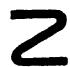
\includegraphics[keepaspectratio]{images/part002_a17f5ac5846160dabe35edfd7ae1b1f71cd54f2b9ab149a24f189ab7736ff1b5.jpg}}

凡涉及序结构、代数结构和拓扑结构时，除非另有明确说明，始终应理解为态射即为上述各例中所定义的态射。

条件 \((MO_{III})\) 且双射的刻画（第二章，§3，第8号，命题8的推论）蕴含以下准则：

CST8. 设 E、E' 为两个集合，每个集合都赋予一个 Σ 型结构。设 f 为从 E 到 E' 的 σ-态射，并设 g 为从 E' 到 E 的 σ-态射。若 g∘f 是 E 到其自身的恒等映射，且 f∘g 是 E' 到其自身的恒等映射，则 f 是 E 到 E' 的同构，且 g 是逆同构。

\pandocbounded{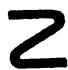
\includegraphics[keepaspectratio]{images/part002_4a2c9e6ca2e0232c08246aaeec85214d3ec9d06a429c17d5fe3c6f33ea15bbf4.jpg}}

应当指出，从E到E'的双射可能是一个σ-态射，而不必要求其逆双射也是σ-态射。* 例如，从拓扑空间A到拓扑空间A'的双射映射可以是连续的，而其逆双射不必是连续的（《一般拓扑学》，第一章，第2节，第1号，注记1）。*

备注。当一类结构 \(\Sigma\) 有多个主基集 \(x_{1},\ldots ,x_{n}\) ，以及辅助基集 \(\mathrm{A}_1,\dots ,\mathrm{A}_m\) ，一个 \(\sigma\) -态射是一个系统 \((f_1,\dots ,f_n)\) ，其中 \(f_{i}\) 是……的映射 \(x_{i}\) 进入。 \(y_{i}(1\leqslant i\leqslant n)\) ，并且这些映射系统满足与（MO \(_{\mathrm{II}}\) ) 和 (MO \(_{\mathrm{III}}\) )，读者可以很容易地自行陈述。

\subsection{更精细的结构}

在本节的其余部分，我们将假设给定了一类结构物种 \(\Sigma\) 以及一个……的概念 \(\sigma\) -态射相对于这类结构；将要引入的所有概念不仅依赖于 \(\Sigma\) 而且还依赖于 \(\sigma\) 通常我们会用“态射”来代替“ \(\sigma\) -态射''。

设 E 是一个集合，并设 \(S_{1}\) , \(S_{2}\) 是 \(\Sigma\) 在 E 上的两个结构。结构 \(S_{1}\) 被称为比 \(S_{2}\) 更细（而 \(S_{2}\) 比 \(S_{1}\) 更粗），如果 E 的恒等映射（从赋有 \(S_{1}\) 的 E 到赋有 \(S_{2}\) 的 E）是一个态射。

当有必要避免歧义时，我们将说 \(G_{1}\) 比……更细 \(G_{2}\) 相对于所考虑的 \(\sigma\) -态射概念；对于本节中将定义的所有其他概念，也类似处理。

假设 \(\mathcal{S}_1\) 比……更细 \(\mathcal{S}_2\) 。如果 \(\mathbf{E}'\) 是一个赋予某种结构的集合 \(\mathcal{S}'\) 的物种 \(\Sigma\) ，并且如果 \(f\) 是……的一个态射 \(\mathbf{E}\) ，赋予 \(\mathcal{S}_2\) 到 \(\mathbf{E}'\) ，赋予 \(\mathcal{S}'\) ，那么 \(f\) 也是 \(\mathbf{E}\) ，赋予 \(\mathcal{S}_1\) 到 \(\mathbf{E}'\) ，赋予 \(\mathcal{S}'\) ；这由前述定义及 \((\mathrm{MO}_{\mathrm{II}})\) 。同样地，如果 \(g\) 是……的一个态射 \(\mathbf{E}'\) ，赋予 \(\mathcal{S}'\) 到 \(\mathbf{E}\) ，赋予 \(\mathcal{S}_1\) ，那么 \(g\) 也是 \(\mathbf{E}'\) ，赋予 \(\mathcal{S}'\) 到 \(\mathbf{E}\) ，赋予 \(\mathcal{S}_2\) .

因此，结构（物种的）越精细 \(\Sigma\) 在E上，以E为源的态射越多，以E为靶的态射就越少。

关系“ \(\mathcal{S}_{1}\) 比……更粗 \(\mathcal{S}_{2}\) ”是……之间的一个序关系 \(\mathcal{S}_{1}\) 并且 \(\mathcal{S}_{2}\) 在所有这些结构的物种的集合上 \(\Sigma\) 在 E 上；因为由 (MO \(_{\text{III}}\) )，由(MO \(_{\text{II}}\) )可传递，且若一个物种结构 \(\Sigma\) 若一个结构既比另一个更细又比另一个更粗，则由（MO \(_{\text{III}}\) ）可知这两个结构相同。按照一般定义（第三章，§1，第14节），定义在E上的两个 \(\Sigma\) 结构被称为可比较的，如果其中一个比另一个更细；一个结构被称为严格更细（相应地，严格更粗）于另一个结构，如果它比另一个更细（相应地，更粗）且与另一个不同。

示例

\begin{enumerate}
\def\labelenumi{(\arabic{enumi})}
\item
  具有图序结构 \(s\) 在集合上 \(A\) 比具有图的序结构更细 \(s'\) 当且仅当 \(s \subset s'\) 。换句话说，关系 \(x \leqslant y\) （关于 \(s\) ）蕴含 \(x \leqslant y\) （关于 \(s'\) ）；这与第三章，§1，第4节，例3中给出的定义一致。
\item
  考虑两个代数结构 F， \(F'\) 同一类型的结构 \(\Sigma\) 在集合 A 上，其中 F 和 \(F'\) 是这两个结构的（处处有定义的）合成法则的图。根据此情形下态射的定义（第1号，例2），F比 \(F'\) 当且仅当 \(F \subset F'\) 更细。但由于F和 \(F'\) 都是具有相同定义域的函数图 \(A \times A\) ，我们必须有 \(F = F'\) 换言之，物种的两个可比较结构 \(\Sigma\) 必然是相同的。
\item
  设 V， \(V'\) 是同一集合A上的两个拓扑。说V比 \(V'\) 意味着，根据此情形下态射的定义（例3，第1条）， \(V' \subset V\) ；换言之，A 的每个在拓扑中为开集的子集 \(V'\) 在拓扑 V 中也是一个开集（因此，拓扑越细，开集就越多）。
\end{enumerate}

注记。我们刚刚遇到了一个例子（例 2），其中两个可比较的同种结构 \(\Sigma\) 必然是相同的。还有许多其他这样的例子：线性序结构、*紧致拓扑、Fréchet空间结构（态射为连续线性映射）、由除环上的绝对值（或赋值）定义的拓扑，等等。*

对于此类结构物种 \(\Sigma\) ，一个态射 \(f\) 从E到E'，若是双射，则是一个同构；因为若我们通过 \(\mathcal{S}\) 将E上的结构 \(f\) 转移到E'上，我们得到一个物种结构 \(\Sigma\) ，它比E'上的结构 \(\mathcal{S}'\) 更细，因此与 \(\mathcal{S}'\) .

\subsection{初始结构}

考虑一个族 \((\mathbf{A}_i)_{i\in \mathbf{I}}\) 集合族，其中每个集合都配备了一个结构 \(\mathcal{S}_i\) 的物种 \(\Sigma\) . 设 \(\mathbf{E}\) 设为一个集合，并且对于每个 \(i\in \mathbf{I}\) 让 \(f_i\) 成为...的映射 \(\mathbf{E}\) 进入。 \(\mathbf{A}_i\) 。一个结构 \(\mathfrak{J}\) ，属于物种 \(\Sigma\) 且位于 \(\mathbf{E}\) 上，被称为关于该族 \((\mathbf{A}_i,\mathcal{S}_i,f_i)_{i\in \mathbf{I}}\) 的一个初始结构，如果它具有以下性质：

（IN）给定任意集合 \(E'\) ，任意结构 \(\mathcal{S}'\) （属于物种 \(\Sigma\) ，在 \(E'\) 上），以及任意从 \(E'\) 到E的映射g，关系

“g 是 \(E'\) 进入。 \(E\)''

的态射”等价于关系“对每个

CST9。若存在关于 \(\iota\in I,f_{\iota}\circ g\) 是……的一个态射 \(E^{\prime}\) 进入。 \(A_{\iota}\) ''.

的初始结构，则它是 \(\mathbf{E}\) 上关于该族 \((\mathbf{A}_t, \mathcal{G}_t, f_t)_{t \in \mathbf{I}}\) 的所有 \(\Sigma\) 在 \(\mathbf{E}\) 上的型结构中余最粗的，其中每个映射 \(f_t\) 都是态射，因此是唯一的。设J是E上的一个初始结构，并设S是E上的一个

型结构，使得每个 \(\Sigma\) 都是态射。若i表示从赋有S的E到赋有J的E的恒等映射，则对一切 \(f_{i}\) ， \(f_{i} \circ i\) 都是态射，且条件(IN)表明i是态射，这意味着（第2节）S比J更细。另一方面，将(IN)应用于g为E（赋有J）到其自身的恒等映射的情形，我们由 \(i \in I\) 可见每个 \((\mathbf{MO}_{\mathbf{III}})\) 都是从E到 \(f_{i}\) 的态射，这完成了证明。 \(A_{i}\) 可能发生这样的情况：存在一个

型结构，即 \(\Sigma\) 在 \(\mathbf{E}\) 上的一个结构，它是所有 \(\Sigma\) 型结构中余最粗的、使每个 \(f_{t}\) 都成为态射的，但该结构并不是关于 \((\mathbf{A}_{t},\mathcal{S}_{t},f_{t})\) 的初始结构（习题6）。我们有以下传递性准则：

是I的一个划分，并设

CST10。设 E 为一个集合，令 \((\mathbf{A}_{\iota})_{\iota\in\mathbf{I}}\) 是一个集合族，并且对每个 \(\iota\in I\) 让 \(G_{\iota}\) 是物种 \(\Sigma\) 在 \(A_{\iota}\) 上的一个结构. 设 \((\mathrm{J}_{\lambda})_{\lambda\in\mathbf{L}}\) 是一个以L为指标集的集合族。对每个 \((\mathrm{B}_{\lambda})_{\lambda\in\mathbf{L}}\) ，设 \(\lambda\in L\) 让 \(h_{\lambda}\) 是从E到 \(B_{\lambda}\) ，并且对于每个 \(\lambda\in L\) 的映射，且对每个 \(\iota\in J_{\lambda}\) 让 \(g_{\lambda\iota}\) 成为...的映射 \(B_{\lambda}\) 进入。 \(A_{\iota}\) ，并且让 \(f_{\iota}=g_{\lambda\iota}\circ h_{\lambda}\) 。假设对每个 \(\lambda\in L\) ，存在一个初始结构 \(G_{\lambda}^{\prime}\) ，位于 \(B_{\lambda}\) 上、关于该族 \((\mathbf{A}_{\iota},\mathcal{G}_{\iota},g_{\lambda\iota})_{\iota\in\mathbf{J}_{\lambda}}\) ，那么以下陈述是等价的：

\begin{enumerate}
\def\labelenumi{(\alph{enumi})}
\item
  存在一个初始结构 \(\mathfrak{J}\) 在 \(\mathbf{E}\) 上，关于该族 \((\mathbf{A}_t, \mathcal{S}_t, f_t)_{t \in \mathbf{I}}\) ;
\item
  存在一个初始结构 \(\mathfrak{J}'\) 在 \(\mathbf{E}\) 上，关于该族 \((\mathbf{B}_{\lambda},\mathcal{S}_{\lambda}^{\prime},h_{\lambda})_{\lambda \in \mathbf{L}}\) .
\end{enumerate}

此外，这些陈述蕴含 \(\mathfrak{J} = \mathfrak{J}'\) .

设 F 是一个赋予物种结构的集合 \(\Sigma\) ，并且让 \(u\) 是 F 到 E 的一个映射。注意根据定义，关系“ \(h_{\lambda} \circ u\) 是 F 到 B 的一个态射 \(_{\lambda}\) ”等价于关系“对所有 \(t \in J_{\lambda}\) , \(g_{\lambda t} \circ h_{\lambda} \circ u = f_{t} \circ u\) 是从 F 到 A 的态射 \(_{t}\) ''。关系

\begin{enumerate}
\def\labelenumi{(\arabic{enumi})}
\tightlist
\item
\end{enumerate}

``对所有 \(\lambda \in \mathbf{L}\) , \(h_{\lambda} \circ u\) 是……的一个态射 \(\mathbf{F}\) 进入。 \(\mathbf{B}_{\lambda}\) ''

因此等价于关系

\begin{enumerate}
\def\labelenumi{(\arabic{enumi})}
\setcounter{enumi}{1}
\tightlist
\item
\end{enumerate}

``对所有 \(\iota\in I,f_{\iota}\circ u\) 是从F到 \(A_{\iota}\) ''.

的态射。现在，说 \(\mathfrak{J}'\) 是关于该族结构的初始结构 \((\mathbf{B}_{\lambda}, \mathcal{S}_{\lambda}', h_{\lambda})_{\lambda \in \mathbf{L}}\) 意味着关系(1)等价于关系“ \(u\) 是……的一个态射 \(F\) 进入。 \(E\) 赋予 \(\mathfrak{J}'\)；并且说 \(\mathfrak{J}\) 是

关于该族系的初始结构 \((\mathbf{A}_{i}, \mathcal{G}_{i}, f_{i})_{i \in I}\) 意味着关系式(2)等价于关系式“u是从F到赋予...的E的态射”。 \(\mathfrak{J}\)因此，根据初始结构唯一性的性质，结论成立。

\subsection{初始结构的例子}

I. 结构的逆像。当 I 是由单个元素组成的集合时，关于 \((\mathbf{A}, \mathcal{G}, f)\) 称为在 f 下结构 G 的原像（当它存在时）。

* 拓扑在任何映射下总有原像 \(f\) ；但对于序结构或代数结构而言，情况并非如此。*

\begin{enumerate}
\def\labelenumi{\Roman{enumi}.}
\setcounter{enumi}{1}
\tightlist
\item
  诱导结构。设 A 是一个赋予某种结构的集合， \(\mathcal{S}\) 的物种 \(\Sigma\) 设 B 是 A 的一个子集，并设 \(j\) 为B到A的典范嵌入。则在 \(j\) 下的原像 \(\mathcal{S}\) （若存在）称为由 \(\mathcal{S}\) 在 B 上。
\end{enumerate}

序结构在其定义集合的每个子集上诱导出同种结构；但对于有向集的结构，情况并非如此。* 拓扑在其定义集合的每个子集上诱导出拓扑，但紧致拓扑一般不会诱导出紧致拓扑。集合A上的代数结构一般不会在任意子集B上诱导出同种结构；如果A上给定的结构由处处有定义的合成律组成，那么B必须对这些律中的每一条都保持稳定，但这个必要条件并不总是充分的。*

一般准则CST10为我们提供了关于诱导结构的如下传递性准则：

CST11。设B是A的子集，C是B的子集，且S是某物种的结构。 \(\Sigma\) 在A上，该结构诱导了一个结构 \(S'\) 同一物种在B上。则S诱导出一个物种结构 \(\Sigma\) 在 C 上当且仅当 \(S'\) 诱导出一个物种结构 \(\Sigma\) 在C上，以及由S和 \(S'\) 则完全相同。

CST12。设 A、A' 为两个赋予结构的集合 \(\mathcal{G}\) , \(\mathcal{S}'\) 的物种 \(\Sigma\) 。设 B 为 A 的子集，B' 为 A' 的子集。假设 \(\mathcal{G}\) （分别） \(\mathcal{G}'\) ) 诱导出物种结构 \(\Sigma\) 在 B（相应地，B'）上。如果 \(f\) 是从A到A'的一个态射，使得 \(f(B) \subset B'\) ，则映射 \(g\) 从 B 到 B' 中，与 \(f\) 在B上是一个态射（关于由 \(\mathcal{G}\) 并且 \(\mathcal{S}'\) ).

让 \(j\) （分别） \(j'\) ）设B（分别地，B'）到A（分别地，A'）的典范嵌入。根据定义，我们有 \(f \circ j = j' \circ g\) 。由于 \(f\) 并且 \(j\) 是态射，所以 \(f \circ j\) 由 \((\mathbf{MO}_{\mathbf{II}})\) 也是；但接着， \(j' \circ g\) 是态射，则映射 \(g\) 根据初始结构的定义是一个态射。

\begin{enumerate}
\def\labelenumi{\Roman{enumi}.}
\setcounter{enumi}{2}
\tightlist
\item
  乘积结构。设 \((\mathbf{A}_t)_{t \in \mathbf{I}}\) 是一族集合，并且在每个集合 \(\mathbf{A}_t\) 让 \(\mathcal{G}_t\) 是物种的一个结构 \(\Sigma\) . 设 \(\mathbf{E} = \prod_{t \in \mathbf{I}} \mathbf{A}_t\) 为这一族的乘积 \((\mathbf{A}_t)_{t \in \mathbf{I}}\) （第二章，第5节），并令 \(\mathbf{pr}_t\) 表示 \(\mathbf{E}\) 到上 \(\mathbf{A}_t\) 的投影。关于该族的初始结构（如果存在） \((\mathbf{A}_t, \mathcal{G}_t, \mathbf{pr}_t)_{t \in \mathbf{I}}\) 称为结构的积 \(\mathcal{G}_t\) .
\end{enumerate}

一族序结构总有积结构，但一族全序结构却并非总是如此。* 一族群结构总有积结构，但一族除环结构却未必如此。一族拓扑总有积结构，但一族局部紧空间结构却并非总是如此；在这种情况下，若族是有限的，则存在同种的积结构，但若族是无限的，则未必存在（参见《一般拓扑学》第一章第9节第7号命题14）。*

准则CST10给出如下关于积结构的结合性准则：

CST13. 设 \((\mathbf{A}_{\iota})_{\iota \in \mathbf{I}}\) 是一个集合族，并且对每个指标 \(\iota \in \mathbf{I}\) 让 \(\mathcal{S}_{\iota}\) 是物种 \(\Sigma\) 在 \(\mathbf{A}_{\iota}\) 上的一个结构. 设 \((\mathrm{J}_{\lambda})_{\lambda \in \mathbf{L}}\) 是……的一个划分 \(\mathbf{I}\) 。假设在每个部分积上 \(\mathbf{B}_{\lambda} = \prod_{\iota \in \mathrm{J}_{\lambda}} \mathbf{A}_{\iota}\) 族 \((\mathcal{S}_{\iota})_{\iota \in \mathrm{J}_{\lambda}}\) 具有一个积结构 \(\mathcal{S}_{\lambda}'\) 。那么族 \((\mathcal{S}_{\iota})_{\iota \in \mathbf{I}}\) 具有一个积结构 \(\mathcal{S}\) 当且仅当族 \((\mathcal{S}_{\lambda}')_{\lambda \in \mathbf{L}}\) 具有一个积结构 \(\mathcal{S}'\) ，并且 \(\mathbf{E} = \prod_{\iota \in \mathbf{I}} \mathbf{A}_{\iota}\) ，赋予 \(\mathcal{S}\) ，映到 \(\mathbf{F} = \prod_{\lambda \in \mathbf{L}} \mathbf{B}_{\lambda}\) ，赋予 \(\mathcal{S}'\) 的典范映射（第二章，§5，第5节）是一个同构。

CST10的另一个应用给出了关于由积结构诱导的结构的如下判据：

CST14. 设 \((\mathbf{A}_{t})_{t\in I}\) 是一个集合族，并且对每个 \(i\in I\) 让 \(\mathcal{S}_i\) 是物种 \(\Sigma\) 在 \(\mathbf{A}_i\) 上的一个结构；对于每一个 \(i\in I\) ，让 \(\mathbf{B}_i\) 为 \(\mathbf{A}_i\) 的一个子集。假设每个 \(\mathcal{S}_i\) 诱导一个结构 \(\mathcal{S}_i'\) 在 \(\mathbf{B}_i\) 上，并且在乘积 \(\mathbf{E} = \prod_{i\in I}\mathbf{A}_i\) 上存在一个结构 \(\mathcal{S}_0\) ，它是族 \((\mathcal{S}_i)\) 的积，那么以下陈述是等价的：

\begin{enumerate}
\def\labelenumi{(\alph{enumi})}
\item
  在集合上 \(\mathbf{B} = \prod_{i\in \mathbf{I}}\mathbf{B}_i\subset \mathbf{E}\) 存在一个结构 \(\mathcal{S}\) 由...诱导的 \(\mathcal{S}_0\)
\item
  的积，在集合B上存在一个结构 \(\mathcal{S}'\) 是结构族 \((\mathcal{S}_t')\) .
\end{enumerate}

此外，这些陈述蕴含 \(\mathcal{S} = \mathcal{S}'\) .

让 \(j_{i}\) 为 \(B_{i}\) 进入。 \(A_{i}\) 的积，设j为B到E的典范单射，设 \(p_{i}\) 为 E 在 \(A_{i}\) ，并且让 \(p_{i}'\) 为 B 在 \(B_{i}\) 上的投影。于是我们有 \(p_{i} \circ j = j_{i} \circ p_{i}'\) 对于所有 \(i \in I\) 。根据CST10， \(\mathcal{G}\) 是关于该族结构的初始结构 \((A_{i}, \mathcal{G}_{i}, p_{i} \circ j)_{i \in I}\) ，以及 \(\mathcal{G}'\) 是关于该族结构的初始结构 \((A_{i}, \mathcal{G}_{i}, j_{i} \circ p_{i}')_{i \in I}\) 。因此结论成立。

逆像与积的概念通过以下判据相联系：

CST15. 设 \((\mathbf{A}_i)_{i\in I}\) 是一个集合族，并且对每个 \(i\in I\) 让 \(\mathcal{S}_i\) 是物种 \(\Sigma\) 在 \(\mathbf{A}_i\) 上的一个结构，并且让 \(f_i\) 为集合 E 到 \(\mathbf{A}_i\) 的一个映射。假设在积集 \(\mathbf{A} = \prod_{i\in I}\mathbf{A}_i\) 上存在一个积结构 \(\mathcal{S}\) ，它是

族 \((\mathcal{S}_t)_{t\in I}\) 的积结构。那么，关于族 \((A_t,\mathcal{S}_t,f_t)_{t\in I}\) 存在一个初始结构，当且仅当结构 \(\mathcal{S}\) 在映射 \(x\to f(x) = (f_t(x))\) （从 E 到 A）下具有逆像，并且此时这两个结构相同。

由于 \(f_{t} = \mathrm{pr}_{t} \circ f\) ，该判据是CST10的一个特例。

备注。设 \((\mathcal{S}_{\lambda})_{\lambda \in L}\) 是物种的一族结构 \(\Sigma\) 在同一集合A上；令 \(A_{\lambda}\) 表示集合A赋予结构 \(\mathcal{S}_{\lambda}\) ，并且让 \(I_{\lambda}\) 表示A到 \(A_{\lambda}\) 的恒等映射。设B为乘积集 \(A^{L} = \prod_{\lambda \in L} A_{\lambda}\) ，并且让 \(\Delta\) 为该乘积的对角线（第二章，

§ 5，第 3 号）。设 h 为 A 到 \(\Delta\) ，因此 \(h(x)\) 的元素 \((x_{\lambda})_{\lambda\in\mathbf{L}}\) 使得 \(x_{\lambda}=x\) 对于所有 \(\lambda\in L\) 。假设在B上存在一个乘积结构 \(G'\) 该族中 \((\mathcal{G}_{\lambda})\) 由于 h 是单射的，准则 CST 15 表明存在一个初始结构 G ，关于该族 \((A_{\lambda},\mathcal{G}_{\lambda},I_{\lambda})_{\lambda\in\mathbf{L}}\) ，当且仅当存在一个结构 \(G''\) 在 \(\Delta\) 上、由 \(G'\) 所诱导； \(G''\) 则与通过 h 将 G 传输到 \(\Delta\) 所得到的结构相同。特别地，当所有结构 \(G_{\lambda}\) 是相同的，则h是A（赋予此结构）到 \(\Delta\) 的一个同构 .

我们还有以下判据：

CST16. 设 \((\mathbf{A}_t)_{t \in \mathbf{I}}\) , \((\mathbf{B}_t)_{t \in \mathbf{I}}\) 为两个由同一集合指标化的集族。对每个 \(t \in \mathbf{I}\) ，让 \(\mathcal{S}_t\) 是物种 \(\Sigma\) 在 \(\mathbf{A}_t\) 上的一个结构，并令 \(\mathcal{S}_t'\) 是物种 \(\Sigma\) 在 \(\mathbf{B}_t\) 上的一个结构。假设在 \(\mathbf{A} = \prod_{t \in \mathbf{I}} \mathbf{A}_t\) （分别地，在 \(\mathbf{B} = \prod_{t \in \mathbf{I}} \mathbf{B}_t\) ) 一个积结构 \(\mathcal{S}\) （分别） \(\mathcal{S}'\) ) 该族的 \((\mathcal{S}_t)\) （分别） \((\mathcal{S}_t')\) ). 对于每一个 \(t \in \mathbf{I}\) ，让 \(f_t\) 为 \(\mathbf{A}_t\) 进入。 \(\mathbf{B}_t\) 。则映射 \(f = (f_t)_{t \in \mathbf{I}}\) 是……的一个态射 \(\mathbf{A}\) 进入。 \(\mathbf{B}\) .

让 \(p_{i}\) （分别） \(q_{i}\) ) 为 A 在 \(A_{i}\) （相应地，B 在 \(B_{i}\) ）上的投影。于是我们有 \(q_{i} \circ f = f_{i} \circ p_{i}\) 。由于 \(f_{i}\) 并且 \(p_{i}\) 是态射（准则

CST9）， \(f_{\iota} \circ p_{\iota}\) 是一个态射，通过 \((\mathbf{MO}_{\mathrm{II}})\) ；因此 \(f\) 由 (IN) 知是态射。

注记。对于大多数常见结构，CST 16 中给出的条件不仅是充分的，而且对于 \(f\) 成为态射（参见练习7）。特别地，在以下情形中确实如此（这些情形会出现，例如，如果 \(\Sigma\) 是序结构的种，* 或群结构的种，或拓扑结构的种 *，等等；参见练习8）：

存在一个族 \((a_{\iota})_{\iota\in I}\) 使得 \(a_{\iota}\in A_{\iota}\) 对于所有 \(\iota \in I\) 并且使得，如果我们令 \(r_\iota(x_\iota) = (y_\kappa)\) ，其中 \(y_{\iota} = x_{\iota}\) 并且 \(y_{\kappa} = a_{\kappa}\) 每当 \(\kappa\neq \iota\) ，每个映射 \(r_\iota\) 是……的一个态射 \(A_{\iota}\) 进入。 \(A\) 。因为如果 \(f = (f_\iota)\) 是……的一个态射 \(A\) 进入。 \(B\) ，我们可以写 \(f_{\iota} = q_{\iota}\circ f\circ r_{\iota}\) 对于所有 \(\iota \in I\) ，并且只需应用 \((MO_{II})\) .

注意， \(r_t\) 是态射，如果满足以下条件：

\begin{enumerate}
\def\labelenumi{(\alph{enumi})}
\tightlist
\item
  对于每个配备了种 \(\Sigma\) 的结构的集合 E，常值映射 \(z \to a_{t}\) 的态射，这完成了证明。 \(\mathbf{A}_{t}\) ；即，对于每个 \(\kappa \in I\) , \(p_{\kappa} \circ r_{t}\) 是……的一个态射 \(\mathbf{A}_{t}\) 进入。 \(\mathbf{A}_{\kappa}\) ，因为当 \(\kappa = t\) ，以及一个常值映射 \(z \to a_{\kappa}\) 当 \(\kappa \neq t\) ；根据积结构的定义， \(r_{t}\) 因此是 \(\mathbf{A}_{t}\) 到A的一个态射。
\end{enumerate}

上述列出的例子不仅满足(a)，还满足以下条件：

\begin{enumerate}
\def\labelenumi{(\alph{enumi})}
\setcounter{enumi}{1}
\tightlist
\item
  在每个集合 \(\mathbf{A}_i' = \mathbf{A}_i \times \prod_{x \neq i} \{a_x\}\) 上，结构 \(\mathcal{S}\) 诱导出一个物种结构 \(\Sigma\) .
\end{enumerate}

设 \(p_{i}^{\prime}\) 表示 \(p_{i}\) 在 \(A_{i}^{\prime}\) 上的限制。如果条件（a）和（b）都满足，则 \(p_{i}^{\prime}\) 是从 \(A_{i}^{\prime}\) 到 \(A_{i}\) 上的同构。事实上， \(p_{i}^{\prime} = p_{i} \circ j_{i}\) ，其中 \(j_{i}\) 是从 \(A_{i}^{\prime}\) 到 \(A\) 的典范注入， \(p_{i}^{\prime}\) 因而由 \((\mathrm{MO}_{\mathrm{II}})\) 可知是态射。另一方面， \(r_{i} = j_{i} \circ (p_{i}^{\prime})^{-1}\) ；因此 \((p_{i}^{\prime})^{-1}\) 是从 \(A_{i}\) 到 \(A_{i}^{\prime}\) 的态射，这是诱导结构定义的直接结论。

最后，我们有以下判据，它在许多情形下刻画了态射：

CST17. 设A和B是两个集合，赋予结构 \(\mathcal{S}_{\mathbf{A}}\) , \(\mathcal{S}_{\mathbf{B}}\) 同一类型的结构 \(\Sigma\) 。假设在 \(\mathbf{A} \times \mathbf{B}\) 该结构 \(\mathcal{S}_{\mathbf{A} \times \mathbf{B}}\) ，即 \(\mathcal{S}_{\mathbf{A}}\) 并且 \(\mathcal{S}_{\mathbf{B}}\) . 设 \(f\) 是A到B的一个映射，设F为其图像，并设 \(\pi\) 为双射 \(x \to (x, f(x))\) 将A映射到F上。然后，对于 \(f\) 要成为从A到B的态射，必要且充分条件是F上应存在一种物种结构。 \(\Sigma\) 由...诱导的 \(\mathcal{S}_{\mathbf{A} \times \mathbf{B}}\) 并且，当F被赋予这个结构时， \(\pi\) 应当是A到F的一个同构。

为了证明充分性，设 \(j\) 为 \(\mathbf{F}\) 进入。 \(\mathbf{A} \times \mathbf{B}\) 的典范嵌入。我们可以写成 \(f = \operatorname{pr}_2 \circ j \circ \pi\) ，以及 \(f\) 根据假设，则是由三个态射复合而成。

为证明必要性，令 \(\mathcal{G}_{\mathbf{F}}\) 为种类 \(\Sigma\) 的结构，它是利用双射将结构 \(\mathcal{G}_{\mathbf{A}}\) 传递到 \(\mathbf{F}\) 上所得，该双射为 \(\pi\) (§1，第5号)。我们必须证明 \(\mathcal{G}_{\mathbf{F}}\) 是 \(\mathcal{G}_{\mathbf{A} \times \mathbf{B}}\) 在 \(\mathbf{F}\) 上诱导的结构。首先注意， \(j\) 是从 \(\mathbf{F}\) 到 \(\mathbf{A} \times \mathbf{B}\) 的态射；事实上， \(j \circ \pi\) 是映射 \(x \to (x, f(x))\) ，它从 \(\mathbf{A}\) 到 \(\mathbf{A} \times \mathbf{B}\) ，并且根据对 \(f\) 的假设及乘积结构的定义是态射；因而由结构的定义可知， \(\mathcal{G}_{\mathbf{F}}, j\) 是态射。还需证明：若 \(\mathbf{E}\) 是赋予种类 \(\Sigma\) 结构的集合， \(g\) 是从 \(\mathbf{E}\) 到 \(\mathbf{F}\) 的映射，且 \(j \circ g\) 是从 \(\mathbf{E}\) 到 \(\mathbf{A} \times \mathbf{B}\) 的态射，则 \(g\) 也是态射；等价地， \(g_{1} = \pi \circ g\) 应是从 \(\mathbf{E}\) 到 \(\mathbf{A}\) 的态射。但 \(g_{1} = \mathrm{pr}_{1} \circ (j \circ g)\) ，因此结论由假设和乘积结构的定义立即得出。

\subsection{最终结构}

考虑一族集合 \((\mathbf{A}_{i})_{i\in I}\) ，每个集合都配备了一个结构 \(\mathcal{G}_i\) 的物种 \(\Sigma\) . 设 \(E\) 设为一个集合，并且对于每个 \(i\in I\) 让 \(g_i\) 成为...的映射 \(\mathbf{A}_i\) 进入。 \(E\) 。一个结构 \(\mathcal{F}\) ，属于物种 \(\Sigma\) 且位于 \(E\) 上，被称为关于该族 \((\mathbf{A}_i,\mathcal{G}_i,g_i)_{i\in I}\) 的最终结构，如果它具有以下性质：

(FI) 给定任意集合 \(\mathbf{E}'\) ，任意结构 \(\mathcal{G}'\) （属于物种 \(\Sigma\) ，在 \(\mathbf{E}'\) 上），以及任意映射 \(f\) 从 \(\mathbf{E}\) 到 \(\mathbf{E}'\) ，关系

“f 是从 E 到 \(E'\)''

的态射”等价于关系“对每个

``对所有 \(\iota\in I,f\circ g_{\iota}\) 是……的一个态射 \(A_{\iota}\) 进入。 \(E'\)''.

CST18. 如果存在关于族 \((\mathbf{A}_{\iota}, \mathcal{S}_{\iota}, g_{\iota})_{\iota \in \mathbf{I}}\) 的 E 上的最终结构，则它是 E 上使得每个映射 \(\Sigma\) 均为态射的 \(g_{\iota}\) 类结构中最细的，因此是唯一的。

让 \(\mathcal{F}\) 是 E 上的最终结构，并设 \(\mathcal{G}\) 是物种的一个结构 \(\Sigma\) 是 E 上使得每个 \(g_{\iota}\) 是一个态射。如果 \(i\) 表示 E 的恒等映射，赋予 \(\mathcal{F}\) 到E上，赋予 \(\mathcal{G}\) ，那么 \(i \circ g_{\iota}\) 对每个 \(\iota \in I\) 。条件 (FI) 于是表明 \(i\) 是一个态射，这意味着（第 2 节） \(\mathcal{G}\) 比……更粗 \(\mathcal{F}\) 。再次将 (FI) 应用于 \(f\) 是 E 的恒等映射（赋予 \(\mathcal{F}\) ）到其自身的情形，我们看到（利用 \((\mathrm{MO}_{\mathrm{III}})\) 都是从E到 \(g_{\iota}\) 是……的一个态射 \(\mathrm{A}_{\iota}\) 到 E 中。这完成了证明。

型结构，它是使得 \(\Sigma\) 在 E 上，它是所有使 \(\Sigma\) 成为态射的 \(g_{i}\) 型结构中最细的，但这个结构并不是关于族 \((\mathbf{A}_{i},\mathcal{G}_{i},g_{i})\) 我们有以下传递性准则：

是I的一个划分，并设

的最终结构。CST19。设 E 是一个集合，设 \((\mathbf{A}_{\iota})_{\iota\in\mathbf{I}}\) 是一个集合族，并且对每个 \(\iota\in I\) 让 \(S_{\iota}\) 是物种 \(\Sigma\) 在 \(A_{\iota}\) 上的一个结构. 设 \((\mathrm{J}_{\lambda})_{\lambda\in\mathbf{L}}\) 是一个以L为指标集的集合族。对每个 \((\mathbf{B}_{\lambda})_{\lambda\in\mathbf{L}}\) ，设 \(\lambda\in L\) ，让 \(h_{\lambda}\) 成为...的映射 \(B_{\lambda}\) 到 E 中；对每个 \(\lambda\in L\) 的映射，且对每个 \(\iota\in J_{\lambda}\) ，让 \(g_{i\lambda}\) 成为...的映射 \(A_{\iota}\) 进入。 \(B_{\lambda}\) ，并放置 \(f_{\iota}=h_{\lambda}\circ g_{i\lambda}\) 。假设对每个 \(\lambda\in L\) ，存在一个最终结构 \(S_{\lambda}^{\prime}\) ，位于 \(B_{\lambda}\) 上、关于该族 \((\mathbf{A}_{\iota},S_{\iota},g_{i\lambda})_{\iota\in\mathbf{J}_{\lambda}}\) ，那么以下陈述是等价的：

\begin{enumerate}
\def\labelenumi{(\alph{enumi})}
\item
  存在一个最终结构 \(\mathcal{F}\) 关于该族在E上 \((\mathbf{A}_i, \mathcal{G}_i, f_i)_{i \in \mathbf{I}}\) .
\item
  存在一个最终结构 \(\mathcal{F}'\) 关于该族在E上 \((\mathbf{B}_{\lambda}, \mathcal{S}_{\lambda}', h_{\lambda})_{\lambda \in \mathbf{L}}\) .
\end{enumerate}

此外，这些命题蕴含 \(\mathcal{F} = \mathcal{F}'\) .

设 F 是一个赋予物种结构的集合 \(\Sigma\) ，并设 u 为从 E 到 F 的映射。根据定义，关系“ \(u \circ h_{\lambda}\) 是……的一个态射 \(B_{\lambda}\) 到 F 中”等价于关系

``对所有 \(\iota\in\mathrm{J}_{\lambda}, u\circ h_{\lambda}\circ g_{i\lambda}=u\circ f_{\iota}\) 是……的一个态射 \(\mathbf{A}_{\iota}\) 进入。 \(\mathbf{F}\)''.

，以及关系

\begin{enumerate}
\def\labelenumi{(\arabic{enumi})}
\setcounter{enumi}{2}
\tightlist
\item
\end{enumerate}

``对所有 \(\lambda \in \mathbf{L}\) , \(u \circ h_{\lambda}\) 是……的一个态射 \(\mathbf{B}_{\lambda}\) 进入。 \(\mathbf{F}''\)

因此等价于关系

\begin{enumerate}
\def\labelenumi{(\arabic{enumi})}
\setcounter{enumi}{3}
\tightlist
\item
\end{enumerate}

``对所有 \(\iota\in I,\quad u\circ f_{i}\) 是……的一个态射 \(A_{\iota}\) 进入。 \(F\)''.

要说 \(\mathcal{F}'\) 是关于该族的最终结构 \((\mathbf{B}_{\lambda},\mathcal{S}_{\lambda}',h_{\lambda})_{\lambda \in \mathbf{L}}\) 这意味着关系(3)等价于关系“ \(u\) 是 E（赋予 \(\mathcal{F}'\) ）到 F'' 的一个态射；而说 \(\mathcal{F}\) 是关于该族的最终结构 \((\mathrm{A}_{\nu},\mathcal{S}_{\nu},f_{\nu})_{\nu \in \mathbf{I}}\) 意味着关系式 (4) 等价于关系式 “ \(u\) 是 E（赋予 \(\mathcal{F}\) 到 F'' 中；因此，根据最终结构的唯一性性质，结论成立。

\subsection{最终结构的例子}

I. 结构的直接像。当 I 是由单个元素组成的集合时，关于 \((\mathbf{A}, \mathcal{S}, f)\) 的最终结构称为结构 G 在 f 下的直接像（当它存在时）。

\begin{enumerate}
\def\labelenumi{\Roman{enumi}.}
\setcounter{enumi}{1}
\tightlist
\item
  商结构。设 A 是赋予物种 \(\Sigma\) 的结构 S 的集合，设 R 是 A 上的等价关系，并设 \(\varphi\) 设φ为A到商集E = A/R上的典范映射（第二章，§6，第2节）。结构S在映射φ下的直接像（当它存在时）称为结构S关于关系R的商结构。
\end{enumerate}

* 一般而言，序结构或代数结构并不对任意等价关系都容许商结构（参见第三章第1节习题2）。另一方面，拓扑总是对任意等价关系容许商结构，但对于豪斯多夫拓扑则未必如此。 *

设 A、B 为两个集合，分别赋予结构 \(\mathcal{S}\) , \(\mathcal{S}'\) 的物种 \(\Sigma\) ，并且让 \(f\) 是A到B的一个态射。设R为等价关系 \(f(x) = f(y)\) ，让 \(\varphi\) 令 为 A 到 A/R 的典范映射，并令 \(j\) 为 \(f(A)\) 到B中。假设 \(\mathcal{S}\) 承认一个商结构 \(\mathcal{S}_0\) 关于R，并且 \(\mathcal{S}'\) 诱导一个结构 \(\mathcal{S}_0'\) 在 \(f(A)\) 上。那么，在典范分解 \(f = j \circ g \circ \varphi\) 的 \(f\) （第二章，§6，第5小节）中，由 \(g\) 给出的、把A/R映到 \(f(A)\) 上且与 \(f\) 相关联的双射，当A/R被赋予 \(\mathcal{S}_0\) 并且 \(f(A)\) 被赋予 \(\mathcal{S}_0'\) 时，是一个态射（但不一定是同构）。因为 \(j \circ g\) 根据商结构的定义是A/R到B的态射，因此 \(g\) 根据诱导结构的定义是A/R到 \(f(A)\)

的态射。 \(\mathcal{S}\) , \(\mathcal{S}'\) 的物种 \(\Sigma\) CST20. 设A，A'为两个带有结构 \(\mathcal{S}_0\) （分别） \(\mathcal{S}_0'\) )的 \(\mathcal{S}\) 的集合，并设R（相应地R'）为A（相应地A'）上的一个等价关系。假设存在一个由R（相应地由R'）得到的商结构 \(\mathcal{S}'\) 。如果 \(f\) 是A到A'的一个态射，且与等价关系R和R'相容，并且 \(g\) 是由 \(f\) 通过取商得到的映射，那么 \(g\) 是A/R到A'/R'的一个态射。

让 \(\varphi\) （分别） \(\varphi'\) ）是A到A/R（相应地A'到A'/R'）的典范映射；于是我们有 \(g \circ \varphi = \varphi' \circ f\) 。由于 \(\varphi'\) 并且 \(f\) 是态射，所以 \(\varphi' \circ f\) 由（MO \(_{II}\) ）。但接着， \(g \circ \varphi\) 作为态射， \(g\) 根据商结构的定义也是态射。

¶ 传递性判据CST19特别地给出以下判据：

CST21. 设A为带有结构 \(\mathcal{S}\) 的物种 \(\Sigma\) 的集合，并设R为A上的一个等价关系，使得在A/R上存在由R得到的商结构 \(\mathcal{S}'\) 的 \(\mathcal{S}\) 。设S为A上的一个比R更粗的等价关系，并设S/R表示A/R上由S得到的商等价关系（第二章，§6，第7小节）。那么存在(A/R)/(S/R)上由S得到的商结构 \(\mathcal{S}''\) 的 \(\mathcal{S}'\) 当且仅当在 A/S 上存在一个商结构 \(\mathcal{S}_0\) 的 \(\mathcal{S}\) ，并且A/S（带有 \(\mathcal{S}_0\) ）到(A/R)/(S/R)（带有 \(\mathcal{S}''\) ）的典范映射是一个同构。

让 \(\varphi\) 令 为 A 到 A/R 的典范映射，并令 \(\psi\) 为A/R到(A/R)/(S/R)的映射。根据CST19， \(\mathcal{G}''\) 是……的商 \(\mathcal{G}'\) 通过S/R当且仅当 \(\mathcal{G}''\) 是关于 (A, \(\mathcal{G}\) , \(\psi \circ \varphi\) ) 的最终结构。该准则随后由以下事实得出：关系 \(\psi(\varphi(x)) = \psi(\varphi(y))\) 等价于 \(S\{x,y\}\).

注记。设 A 为赋予了一个结构的集合 \(\mathcal{G}\) 的物种 \(\Sigma\) ，并设 R 是 A 上的一个等价关系，使得在 E = A/R 上存在一个商结构 \(\mathcal{G}'\) 的 \(\mathcal{G}\) 由 R 给出。设 \(\varphi\) 为 A 到 E 的典范映射。一般而言，不存在截面 \(s\) 的 \(\varphi\) （第二章，§3，第 8 号）是 E 到 A 的态射。假设这样的截面 \(s\) 存在，并且进一步假设存在一个结构 \(\mathcal{G}''\) ，由 \(\mathcal{G}\) 在 \(s(E)\) 上诱导。那么，若 \(j\) 表示 \(s(E)\) 到 A 的典范单射，且若 \(s = j \circ f\) ，双射 \(f\) 是 E 到 \(s(E)\) 的一个同构。因为 \(f\) 由诱导结构的定义是一个态射，而 \(g = \varphi \circ j\) 是……的一个态射 \(s(E)\) 到 E 的映射由于 \((MO_{II})\) 。由于 \(g \circ f\) 并且 \(f \circ g\) 分别是 E 和 \(s(E)\) 的恒等映射，该断言是 CST8 的推论。

\section{泛映射}

\subsection{全集与映射}

让 \(\mathfrak{G}\) 是一个比集合论更强的理论，并令 \(\mathbf{E}\) 是...中的一项 \(\mathfrak{G}\) . 设 \(\Sigma\) 成为结构的一个种类，在 \(\mathfrak{G}\) 为简单起见，我们将在全文中假设 \(\Sigma\) 定义在单个（主）基集上，并且为简洁起见，我们将称“ \(\Sigma\) -集”为“赋予物种结构 \(\Sigma\) 的集合”。此外，我们假设 \(\sigma\) -态射已为物种定义 \(\Sigma\) ( \(\S 2\) ，第1号；如同在 \(\S 2\) 中，我们将用“态射”代替“ \(\sigma\) -态射”）。最后，物种 \(\Sigma\) 定义在基集上 \(x\) 并且具有 \(s\) 作为一般结构（ \(\S 1\) ，第4号），让我们假设一个项 \(\alpha \{x, s\}\) 在 \(\mathfrak{G}_{\Sigma}\) 中被定义，满足以下条件：

\((\mathbf{Q}\mathbf{M}_{\mathbf{I}})\) ，以及关系 \(\alpha \{x,s\} \subset \mathcal{F}(\mathbf{E};x)\) 在 \(\mathfrak{C}_{\Sigma}\) .

（QM \(_{II}\) ）如果在（一个理论 \(\mathfrak{G}'\) 该理论强于 \(\mathfrak{G}\) 中）F和F'是两个赋予结构的集合 \(\mathscr{S}\) , \(\mathscr{G}'\) 的物种 \(\Sigma\) ，且若 f 是 F 到 F' 的一个态射，则关系 \(\varphi \in \alpha \{F, \mathscr{G}\}\) 的极大性可知 \(f \circ \varphi \in \alpha \{F', \mathscr{G}'\}\) .

我们将这一关系表述为 \(\varphi\in\alpha\{x,s\}\) 通过说 \(\varphi\) 是 \(\alpha\) 从E到 \(x\) （赋予 \(s\) ).

一个 \(\Sigma\) -集合 \(\mathbf{F}_{\mathbf{E}}\) 和一个 \(\alpha\) -映射 \(\varphi_{\mathbf{E}}\) 的 \(\mathbf{E}\) 进入。 \(\mathbf{F}_{\mathbf{E}}\) 被称为万有的，如果满足以下条件：

(AU) 对每个 \(\alpha\) -映射 \(\varphi\) 的 \(\mathbf{E}\) 到 \(\Sigma\) -集合 \(\mathbf{F}\) 中存在唯一的态射 \(f\) 的 \(\mathbf{F}_{\mathbf{E}}\) 进入。 \(\mathbf{F}\) 使得 \(\varphi = f \circ \varphi_{\mathbf{E}}\) .

对 \((\mathbf{F}_{\mathbf{E}}, \varphi_{\mathbf{E}})\) 于是也称其为 E 的泛映射问题（相对于 \(\Sigma\) , \(\sigma\) ，以及 \(\alpha\) ).

让 \((\mathbf{F}_{\mathbf{E}}^{\prime},\varphi_{\mathbf{E}}^{\prime})\) 并且 \((\mathbf{F}_{\mathbf{E}}^{\prime \prime},\varphi_{\mathbf{E}}^{\prime \prime})\) 是 E 的泛映射问题的两个解。条件 (AU) 表明，存在唯一的态射 \(f_{1}\) 的 \(\mathbf{F}_{\mathbf{E}}^{\prime}\) 进入。 \(\mathbf{F}_{\mathbf{E}}^{\prime \prime}\) 和唯一的态射 \(f_{2}\) 的 \(\mathbf{F}_{\mathbf{E}}^{\prime \prime}\) 进入。 \(\mathbf{F}_{\mathbf{E}}^{\prime}\) 使得 \(\varphi_{\mathbf{E}}^{\prime \prime} = f_{1}\circ \varphi_{\mathbf{E}}^{\prime}\) 并且 \(\varphi_{\mathbf{E}}^{\prime} = f_{2}\circ \varphi_{\mathbf{E}}^{\prime \prime}\) 。因此我们有 \(\varphi_{\mathbf{E}}^{\prime} = f_{2}\circ f_{1}\circ \varphi_{\mathbf{E}}^{\prime}\) 并且 \(\varphi_{\mathbf{E}}^{\prime \prime} = f_{1}\circ f_{2}\circ \varphi_{\mathbf{E}}^{\prime \prime}\) 。将(AU)应用于 \(\mathbf{F} = \mathbf{F}_{\mathbf{E}}^{\prime}\) 并且 \(\varphi = \varphi_{\mathbf{E}}^{\prime}\) 的情形，我们得出 \(f_{2}\circ f_{1}\) 是 \(\mathbf{F}_{\mathbf{E}}^{\prime}\) 到自身的恒等映射。类似地， \(f_{1}\circ f_{2}\) 是 \(\mathbf{F}_{\mathbf{E}}^{\prime \prime}\) 到自身。因此（§2，第1号，准则CST8）， \(f_{1}\) 是……的一个同构 \(\mathbf{F}_{\mathbf{E}}^{\prime}\) 到上 \(\mathbf{F}_{\mathbf{E}}^{\prime \prime}\) ，以及 \(f_{2}\) 是它的逆同构。这个结果表述为：E的泛映射问题的解在同构意义下是唯一的。

为了验证一个对 \((\mathbf{F}_{\mathbf{E}}, \varphi_{\mathbf{E}})\) 是E的泛映射问题的一个解，通常方便的做法是验证以下两个条件：

（AU \(_{I}'\) ）对于每个Σ-集F和每个从E到F的α-映射φ，存在一个从F \(_{E}\) 到F的态射f，使得φ = f∘φ \(_{E}\) .

（AU \(_{II}'\) ）对于每个Σ-集F，两个从F \(_{E}\) 到F且在φ \(_{E}\) （E）上一致的态射相等。

因为如果这两个条件被满足，则由 \(f\) 所保证其存在的态射 \((\mathbf{AU}_{\mathbf{I}}^{\prime})\) 是唯一的，由 \((\mathbf{AU}_{\mathbf{II}}^{\prime})\) 。反之，显然(AU)蕴含 \((\mathbf{AU}_{\mathbf{I}}^{\prime})\) ；此外，如果 \(f\) 并且 \(f'\) 是 \(\mathbf{F}_{\mathbf{E}}\) 进入。 \(\mathbf{F}\) 的两个态射，它们在 \(\varphi_{\mathbf{E}}(\mathbf{E})\) ，我们有 \(f \circ \varphi_{\mathbf{E}} = f' \circ \varphi_{\mathbf{E}}\) ，由此 \(f = f'\) 上一致，则将(AU)应用于 \(\alpha\) -映射 \(f \circ \varphi_{\mathbf{E}}\) 。因此(AU)蕴含 \((\mathbf{AU}_{\mathbf{II}}^{\prime})\) .

\subsection{泛映射的存在性}

一个泛映射问题不一定有解（习题1）。然而，我们将证明以下条件蕴含解的存在性：

\((\mathbf{CU}_{\mathbf{I}})\) 在每一族 \(\Sigma\) -集合的乘积上，存在一个物种 \(\Sigma\) 的乘积结构（§2，第4节）。

\((\mathrm{CU}_{\mathrm{II}})\) 让 \((\mathbf{F}_i)_{i\in \mathbf{I}}\) 是 \(\Sigma\) -集的族，且对每个 \(i\in I\) 让 \(\varphi_i\) 是 \(\alpha\) 从E到 \(\mathbf{F}_i\) 。则映射 \((\varphi_i)_{i\in I}\) 将E映入 \(\prod_{i\in I}F_i\) （赋予乘积结构）是一个 \(\alpha\) -映射。

一个 \(\Sigma\) -集合 F 的子集 G 被称为 \(\Sigma\) -可容许的，如果 F 上的结构在 G 上诱导出一个物种结构 \(\Sigma\) （ \(\S\) 2，第 4 期）。

（CU \(_{III}\) 存在一个基数 \(\mathfrak{a}\) 具有以下性质：对于每一个 \(\Sigma\) -集合 \(\mathbf{F}\) 以及每一个 \(\alpha\) -映射 \(\varphi\) 的 \(\mathbf{E}\) 进入。 \(\mathbf{F}\) 存在一个 \(\Sigma\) -容许子集 \(\mathbf{G}\) 的 \(\mathbf{F}\) 它包含 \(\varphi(\mathbf{E})\) ，具有基数 \(\leqslant \mathfrak{a}\) ，使得 \(\mathbf{E}\) 进入。 \(\mathbf{G}\) 的映射具有与 \(\varphi\) 是 \(\alpha\) -映射，并且使得任意两个 \(\mathbf{G}\) 到 \(\Sigma\) -集合的态射，若它们在 \(\varphi(\mathbf{E})\) 是相等的。

CST22。如果条件 \((\mathrm{CU}_{\mathrm{I}})\) 至 \((\mathrm{CU}_{\mathrm{III}})\) 均成立，那么 E 的泛映射问题有解。

我们首先证明，如果存在一对 \((\mathbf{F}_{\mathbf{E}}, \varphi_{\mathbf{E}})\) 满足 \((\mathbf{AU}_{\mathbf{I}}^{\prime})\) ，那么对于 E 的泛映射问题也存在一个解。因为通过 \((\mathrm{CU}_{\mathrm{III}})\) 存在一个 \(\Sigma\) -容许子集 \(F_{E}^{\prime}\) 的 \(F_{E}\) 包含 \(\varphi_{E}(E)\) ，使得映射 \(\varphi_{E}^{\prime}\) 将E映入 \(F_{E}^{\prime}\) 其图与 \(\varphi_{E}\) 是 \(\alpha\) -映射，并且使得任意两个 \(F_{E}^{\prime}\) 到 \(\Sigma\) 在……上一致的集合 \(\varphi_{E}(E)\) 相等。设 j 为……的典范嵌入 \(F_{E}^{\prime}\) 进入。 \(F_{E}\) ，因此 \(\varphi_{E} = j \circ \varphi_{E}^{\prime}\) 。对于每一个态射 f，从 \(F_{E}\) 到 \(\Sigma\) -集合 F， \(f \circ j\) 是……的一个态射 \(F_{E}^{\prime}\) 到 F 中，并且我们有 \(f \circ \varphi_{E} = (f \circ j) \circ \varphi_{E}^{\prime}\) 。因此显然 \((\mathbf{F}_{\mathbf{E}}^{\prime}, \varphi_{\mathbf{E}}^{\prime})\) 满足 \((\mathbf{AU}_{\mathbf{I}}^{\prime})\) 并且 \((\mathbf{AU}_{\mathbf{II}}^{\prime})\) .

我们只需证明这样一个对子的存在性。 \((\mathrm{F}_{\mathbf{E}}, \varphi_{\mathbf{E}})\) 满足 \((\mathrm{AU}_{\mathbf{I}}^{\prime})\) . 设 \(s \in \mathrm{S}(x)\) 成为结构种类的典型刻画 \(\Sigma\) ，并考虑子集 L，它由 \(\mathfrak{P}(\mathfrak{a}) \times \mathrm{S}(\mathfrak{a}) \times \mathfrak{P}(\mathbf{E} \times \mathfrak{a})\) 中的所有三元组构成 \(\lambda = (\mathbf{X}, \mathbf{V}, \mathbf{P})\) 具有以下性质：“V是物种 \(\Sigma\) 在 \(X \subset a\) 上的一个结构，且 P 是某个 \(\alpha\) -映射（将E映射到X，关于结构V）的图''

（注意我们有 \(S(X) \subset S(a)\) ，这可以通过对阶梯构造方案的步骤长度逐步论证而容易看出 \(S\) ）。对于每个 \(\lambda = (X, V, P) \in L\) ，我们用 \(X_{\lambda}\) 集合 \(X\) 表示赋予结构 \(V\) 的集合，并用 \(\varphi_{\lambda}\) 表示 \(E\) 进入。 \(X_{\lambda}\) 其图形为 \(P\) .

让 \(F_{E}\) 是 \(\Sigma\) -集的映射，该映射是 \(X_{\lambda}\) 的乘积（它由 \((CU_{I})\) ），并令 \(\varphi_{E}\) 为映射 \(x \to (\varphi_{\lambda}(x))\) 将E映入 \(F_{E}\) ，这是一个 \(\alpha\) 根据 \((CU_{II})\) 的映射。让我们证明这一对 \((F_{E}, \varphi_{E})\) 满足 \((AU_{I}')\) 。给定一个从 E 到某个 \(\alpha\) -映射 \(\varphi\) -集合 F 的 \(\Sigma\) ，设 G 是 F 的一个子集，它满足 \((CU_{III})\) 中所述的条件。令 j 为 G 到 F 的典范嵌入，并令 \(\psi\) 为从 E 到 G 的映射，其图像与 \(\varphi\) ，因此 \(\varphi = j \circ \psi\) 相同。由此可知， \((CU_{III})\) 蕴含 \(\psi\) 是一个 \(\alpha\) -映射，从 E 到 G。由于 Card \((G) \leqslant a\) ，存在一个与 G 等势的子集 \(G'\) ，它包含于某个与 G 等势的集合中。设 g 为从 G 到 \(G'\) 如果我们通过 g 将物种结构 \(\Sigma\) 传输到 G 上，那么根据定义存在一个 \(\lambda\) L 中的元素，使得 \(G'\) （带有传输结构）等于 \(X_{\lambda}\) 并且使得 \(g \circ \psi = \varphi_{\lambda}\) 。然后 \(f = j \circ \overline{g}^1 \circ \mathrm{pr}_{\lambda}\) 是……的一个态射 \(\mathbf{F}_{\mathbf{E}}\) 进入。 \(\mathbf{F}\) 使得 \(\varphi = f \circ \varphi_{\mathbf{E}}\) ，证明完成。

CST23. 设 \((\mathbf{F}_{\mathbf{E}}, \varphi_{\mathbf{E}})\) 为 E 的泛映射问题的一个解。那么 \(\varphi_{E}\) 是 E 到 \(F_{E}\) 的单射，当且仅当对于 E 中每一对不同的元素 x, y，存在一个 \(\alpha\) -映射 \(\varphi\) -集合 F 的 \(\Sigma\) -集 F 使得 \(\varphi(x) \neq \varphi(y)\) .

由于 \(\varphi_{E}\) 是 \(\alpha\) -映射，该判据是定义的直接推论。

在这种情况下， \(\alpha\) -映射被称为分离E的元素，并且我们在术语上通常不区分E的元素与其在 \(\varphi_{E}\) 下的像。按照这一约定，如果 \((F_{E}, \varphi_{E})\) 是某个泛映射问题的解，并且如果条件 \((CU_{III})\) 被满足，那么每一个从E到某个 \(\alpha\) -集合F的 \(\Sigma\) -映射都唯一地延拓为从 \(F_{E}\) 到F的一个态射。

\subsection{泛映射的实例}

* 以下示例大多将在本系列的其他部分详细讨论。

I. 自由代数结构。设 E 为一个集合，且令 \(\Sigma\) 设代数结构的一个种，由一种或多种合成法则定义。我们取该种的同态作为态射。 \(\Sigma\) 所考虑的，以及作为 \(\alpha\) -映射为从 E 到某个 \(\Sigma\) -集的任意映射（换言之， \(\alpha\{x, s\} = \mathcal{F}(E, x)\) ）。所有常见的代数结构种类都满足 \((\mathrm{CU}_{\mathrm{III}})\) ；除了可除环结构之外，它们还满足 \((\mathrm{CU}_{\mathrm{I}})\) ，以及 \((\mathrm{CU}_{\mathrm{II}})\) 这里是……的一个平凡推论 \((\mathrm{CU}_{\mathrm{I}})\) .

由于一般情况下存在物种的结构 \(\Sigma\) 定义在至少包含两个元素的集合上， \(\alpha\) -映射将E的元素分开，因此E可被视为嵌入到 \(F_{E}\) . \(F_{E}\) 被称为由E生成的自由 \(\Sigma\) -集合。因此在代数中，我们谈论自由半群、自由群、自由模和自由代数。

\begin{enumerate}
\def\labelenumi{\Roman{enumi}.}
\setcounter{enumi}{1}
\item
  分式环与分式域。设E为含单位元的交换环，并设S为E中不包含0的乘法封闭子集。我们取 \(\Sigma\) 设为带单位元的交换环的结构类，态射为将单位元映到单位元的环同态。 \(\alpha\) 映射将为同态 \(\varphi\) ，将E映入带单位元的交换环A，使得 \(\varphi(1)=1\) 并且 \(\varphi(S)\) 仅包含A中的单位。条件 \((\mathbf{Q}\mathbf{M}_{\mathbf{II}}), (\mathbf{C}\mathbf{U}_{\mathbf{I}})\) 通过 \((\mathbf{C}\mathbf{U}_{\mathbf{III}})\) （与 \(\mathfrak{a}=\operatorname{Card}(\mathbf{E})\operatorname{Card}(\mathbf{N}))\) 立即得到验证。因此，泛映射问题总有解。 \((\mathbf{F}_{\mathbf{E}},\varphi_{\mathbf{E}})\) ，但一般而言 \(\varphi_{E}\) 不是单射的。最常出现的情形是E为整环；在这种情况下， \(\varphi_{E}\) 是单射的。此外，如果我们取 \(S = E - \{0\}\) ，那么 \(F_{E}\) 是一个域，称为E的分式域。
\item
  两个模的张量积。设 E 为两个模 A × B 在具有单位元的交换环 C 上的乘积。取 Σ 为 C-模结构的种类，态射为线性映射，α-映射为从 A × B 到某个 C-模的双线性映射。条件 (QM \(_{II}\) ）显然被满足，（CU \(_{I}\) ）到（CU \(_{III}\) ）亦然（其中 a = Card (E) Card (C) Card (N)）。对应于对 (A, B) 的泛 C-模 F \(_{E}\) 称为 A 与 B 的张量积，记作 A ⊗ B。泛映射 φ \(_{E}\) 记作 (x, y) → x ⊗ y；它是双线性的，但一般不是单射。
\item
  模的算子环的扩张。设 A 为带单位元的交换环，B 为 A 的包含 A 的单位元的子环，E 为 B-模。该种 \(\Sigma\) 是 A-模结构的种，态射为 A-线性映射，而 \(\alpha\) -映射为 E 到 A-模的 B-线性映射。对应于 B-模 E 的泛 A-模 \(F_{E}\) 称为将 E 的算子环 B 扩张到 A 而得到的模。
\end{enumerate}

V. 一致空间的完备化。设 E 为一个一致空间。取 \(\Sigma\) 为完备 Hausdorff 一致空间结构的种，态射为一致连续映射，而 \(\alpha\) -映射为 E 到完备 Hausdorff 一致空间的一致连续映射。此处完备 Hausdorff 一致空间的 \(\Sigma\) -容许子集为闭子集（关于空间的拓扑），且条件 \((\mathrm{QM}_{\mathrm{II}})\) 并且 \((\mathrm{CU}_{\mathrm{I}})\) 通过 \((\mathrm{CU}_{\mathrm{III}})\) 被满足（其中 \(a = 2^{2^{\operatorname{Card}(E)}}\) ）。完备 Hausdorff 一致空间（在同构意义下）是与 E 相关联的 Hausdorff 一致空间的完备化（《一般拓扑学》第二章，第3节，第7号）。

\begin{enumerate}
\def\labelenumi{\Roman{enumi}.}
\setcounter{enumi}{5}
\item
  Stone-Čech 紧化。设 E 为一个完全正则空间。 \(\Sigma\) 是紧致空间结构的物种，态射为连续映射（从一个紧致空间到另一个紧致空间），且 \(\alpha\) -映射是将E映入紧空间的连续映射。 \(\Sigma\) -可容许子集再次是闭子集，且条件 \((\mathrm{QM}_{\mathrm{II}})\) , \((\mathrm{CU}_{\mathrm{I}})\) 通过 \((\mathrm{CU}_{\mathrm{III}})\) 容易验证（基数与例V中的相同）。紧空间 \(F_{E}\) 是（在同构意义下）通过关于使E到区间的所有连续映射一致的最粗一致性完备化E而得到的“Stone-Čech紧化”。 {[}0, 1{]} R上的映射是一致连续的（一般拓扑学，第九章，§1，习题7）；映射 \(\varphi_{E}\) 是单射的，因为E中任意两个不同的点都可以通过E到 {[}0, 1{]}.
\item
  自由拓扑群。设E为完全正则空间，设 \(\Sigma\) 为豪斯多夫拓扑群结构的范畴，其态射为连续同态；并取 \(\alpha\) -映射为从 E 到豪斯多夫拓扑群的连续映射。条件（ \(QM_{II}\) ）和（ \(CU_{I}\) ）到（ \(CU_{III}\) 容易验证，
\end{enumerate}

\[
\mathfrak {a} = \text { Card } (\mathbf {E}) \text { Card } (\mathbf {N}).
\]

豪斯多夫拓扑群 \(F_{E}\) 它是E的这个泛映射问题的解，称为由空间E生成的自由拓扑群。由于E的任意两个不同点可以通过E到豪斯多夫拓扑群R的连续映射分离，映射 \(\varphi_{E}\) 是单射；可以证明 \(\varphi_{E}\) 是从 E 到子空间 \(\varphi_{\mathrm{E}}(\mathrm{E})\) 的 \(F_{E}\) (*) 的同胚。我们不取 \(\Sigma\) 作为豪斯多夫拓扑群的结构种，我们也可以采用其他结构种，例如豪斯多夫拓扑阿贝尔群、紧群、豪斯多夫拓扑环、豪斯多夫拓扑向量空间（在拓扑除环上，将其视为辅助基集）等。

\begin{enumerate}
\def\labelenumi{\Roman{enumi}.}
\setcounter{enumi}{7}
\item
  关于拓扑群上的概周期函数。设E为一个拓扑群。取 \(\Sigma\) 作为紧致群结构的范畴，其态射为连续同态，且 \(\alpha\) -映射为从 E 到紧群的连续同态。条件 (QM \(_{II}\) ), (CU \(_{I}\) ）到（CU \(_{III}\) ) 被满足，且 \(a = 2^{2^{\text{Card(E)}}}\) . 紧群 F \(_{E}\) 它是E的这个泛映射问题的解，称为与E相联系的紧群；该映射 \(\varphi_{E}\) 不一定是单射的。E 上每个形如 \(g \circ \varphi_{E}\) ，其中 g 是定义在 \(F_E\)，被称为 E 上的概周期函数。
\item
  阿尔巴尼斯簇。设E是一个代数簇，令 \(\Sigma\) 设为与E同基域的阿贝尔簇结构物种（阿贝尔簇是带有代数群结构的完备代数簇；它必然是交换的）。态射是从一个阿贝尔簇到另一个阿贝尔簇的有理映射（每个态射必然是同态与平移的复合）。 \(\alpha\) -映射是从E到阿贝尔簇的有理映射。条件（CU \(_{I}\) 不满足，然而这个关于 E 的泛映射问题却存在一个解 \(F_{E}\) ，称为 E 的 Albanese 簇。一般地，有理映射 \(\varphi_{E}\) 并非单射。*
\end{enumerate}

\startexercises

\exercisegroup

\begin{enumerate}
\def\labelenumi{\arabic{enumi}.}
\tightlist
\item
  设 S 为符号 P, X, 的集合， \(x_{1}, \ldots, x_{n}\) ，这些字母 \(x_{i}\) 权重为0，P权重为1，X权重为2。设T为L(S)中的一个平衡词。这样的词将被称为上的梯队类型 \(x_{1}, \ldots, x_{n}\) .
\end{enumerate}

让 \(\mathbf{E}_1, \ldots, \mathbf{E}_n\) 是 \(n\) 理论中比集合论更强的项。对于每个层级类型 \(\mathbf{T}\) （在 \(x_1, \ldots, x_n\) 上），如下定义项 \(\mathbf{T}(\mathbf{E}_1, \ldots, \mathbf{E}_n)\) ：

\begin{enumerate}
\def\labelenumi{(\roman{enumi})}
\item
  如果 \(\mathbf{T}\) 是一个字母 \(x_{i}\) ，那么 \(\mathbf{T}(\mathbf{E}_{1},\ldots,\mathbf{E}_{n})\) 是集合 \(\mathbf{E}_i\) .
\item
  如果 \(\mathbf{T}\) 具有形式 \(\mathsf{PU}\) ，那么 \(\mathbf{T}(\mathbf{E}_1, \ldots, \mathbf{E}_n)\) 是集合
\end{enumerate}

\[
\mathfrak {P} (\mathrm{U} (\mathrm{E} _ {1}, \dots , \mathrm{E} _ {n})).
\]

\begin{enumerate}
\def\labelenumi{(\roman{enumi})}
\setcounter{enumi}{2}
\tightlist
\item
  如果T具有XUV的形式，其中U和V是T的前驱组装，则 \(\mathrm{T}(\mathrm{E}_{1},\ldots,\mathrm{E}_{n})\) 是集合 \(\mathrm{U}(\mathrm{E}_{1},\ldots,\mathrm{E}_{n})\times\mathrm{V}(\mathrm{E}_{1},\ldots,\mathrm{E}_{n})\) 。证明，对于每个关于 \(x_{1},\ldots,x_{n}\) , \(\mathrm{T}(\mathrm{E}_{1},\ldots,\mathrm{E}_{n})\) 是各项上的阶梯形 \(E_{1},\ldots,E_{n}\) ，反之亦然（通过对阶梯类型长度或阶梯构造方案长度进行归纳证明）。 \(\mathrm{T}(\mathrm{E}_{1},\ldots,\mathrm{E}_{n})\) 被称为阶梯类型T在项上的实现 \(E_{1},\ldots,E_{n}\) 更精确地说，n 个不同字母上的每个梯队都可以唯一地写成如下形式 \(\mathrm{T}(x_{1},\ldots,x_{n})\) ，其中 T 是一个梯队类型。
\end{enumerate}

还说明如何将 n 个映射与 n 个字母上的梯队类型 T 关联起来 \(f_{1}, \ldots, f_{n}\) ，并给出这些映射的一个典范扩张。由此推出，如果 n 个字母上的两个梯队构造方案 S， \(S'\) 满足 \(\mathrm{S}(x_{1}, \ldots, x_{n}) = \mathrm{S}'(x_{1}, \ldots, x_{n}) (x_{1}, \ldots, x_{n} \text{ 为互不相同的字母})\) ，那么 \(\langle f_{1}, \ldots, f_{n} \rangle^{S} = \langle f_{1}, \ldots, f_{n} \rangle^{S'}\) .

\exercisegroup

\begin{enumerate}
\def\labelenumi{\arabic{enumi}.}
\tightlist
\item
  设 S 为符号 P、P-、X、X- 的集合， \(x_1, \ldots, x_n\) ，这些字母 \(x_i\) 权重为0，P和P-权重为1，X、X-权重为2。对于L(S)中的每个词A，我们如下定义A的方差：每个字母 \(x_i\) ，并且符号 P、X 的方差为 0；符号 P⁻、X⁻ 的方差为 1；A 的方差是 A 中出现的符号的方差之和 *（在域 F₂ 中）*（换句话说，如果 A 包含偶数个方差为 1 的符号，则为 0，否则为 1）。
\end{enumerate}

一个有符号阶梯型是L(S)中的一个平衡词A（第一章，附录，第3节），它满足以下两个条件之一：（1）A是其中一个字母 \(x_i\) ； (2) 若 A 具有形式 \(f\mathbf{A}_1\mathbf{A}_2 \ldots \mathbf{A}_p\) (第一章，附录，第3号，命题2的推论2)，其中 \(f\) 是其中一个标志 \(\mathsf{P}, \mathsf{P}^{-}, \mathsf{X}, \mathsf{X}^{-}, p\) 等于1或2，且 \(\mathbf{A}_i\) ( \(1 \leqslant i \leqslant p\) )是平衡词，则每一个 \(\mathbf{A}_i\) 是带符号阶梯型；进一步，若 \(f = \mathsf{X}\) ，那么 \(\mathbf{A}_1\) 并且 \(\mathbf{A}_2\) 的方差为0，且若 \(f = \mathsf{X}^{-}\) ，那么 \(\mathbf{A}_1\) 并且 \(\mathbf{A}_2\) 方差为1。

一个带符号的阶梯型被称为协变的，如果它的方差为0；被称为逆变的，如果它的方差为1。如果在带符号的阶梯型A中，分别将P-和X-替换为P和X，我们得到阶梯型A*（§1，练习1）。阶梯型A*在n个项E₁上的每一个实现， \ldots，Eₙ 称为符号阶梯型 A 在 E₁ 上的一个实现， \ldots，Eₙ，并记为 A(E₁， \ldots，Eₙ）。

让 \(\mathbf{E}_1, \ldots, \mathbf{E}_n, \mathbf{E}_1', \ldots, \mathbf{E}_n'\) 是集合，并令 \(f_i\) 成为...的映射 \(\mathbf{E}_i\) 进入。 \(\mathbf{E}_i'\) ( \(1 \leqslant i \leqslant n\) ）。证明：对每个定义在 \(x_1, \ldots, x_n\) 上的带符号阶梯型 S，我们可以关联一个映射 \(\{f_1, \ldots, f_n\}^{S}\) 满足以下性质：

\begin{enumerate}
\def\labelenumi{(\roman{enumi})}
\item
  如果S是协变的（相应地，逆变的），那么 \(\{f_1, \ldots, f_n\}^{S}\) 是……的映射 \(\mathrm{S}(\mathrm{E}_1, \ldots, \mathrm{E}_n)\) 进入。 \(\mathrm{S}(\mathrm{E}_1', \ldots, \mathrm{E}_n')\) （分别为 \(\mathrm{S}(\mathrm{E}_1', \ldots, \mathrm{E}_n')\) 进入。 \(\mathrm{S}(\mathrm{E}_1, \ldots, \mathrm{E}_n)\) ).
\item
  如果 S 是一个字母 \(x_{i}\) ，那么 \(\{f_1, \ldots, f_n\}^{S}\) 是 \(f_{i}\) .
\item
  若S是PT（相应地，P-T），且若 \(g = \{f_1, \ldots, f_n\}^{\mathrm{T}}\) 是F到 \(\mathbf{F}'\) ，那么 \(\{f_1, \ldots, f_n\}^{S}\) 是 \(g\) 到子集集合的扩展（分别是 \(\overline{g}^1\) 到子集的集合。
\item
  如果 S 是 XTU 或 X-TU，如果 \(\{f_{1},\ldots,f_{n}\}^{T}\) 是一个映射 \(g:F\to F'\) 并且如果 \(\{f_{1},\ldots,f_{n}\}^{U}\) 是一个映射 \(h:G\to G'\) ，那么 \(\{f_{1},\ldots,f_{n}\}^{S}\) 是扩展 \(g\times h:F\times G\to F'\times G'\) .
\end{enumerate}

该映射 \(\{f_1, \ldots, f_n\}^{S}\) 被称为的带符号典范扩张 \(f_1, \ldots, f_n\) 对应于带符号的阶梯型S。若S是一个阶梯型（即，若 \(\mathbb{P}^{-}\) 并且 \(\mathbb{X}^{-}\) 不出现在 S 中），则带符号的典范扩张 \(\{f_1, \ldots, f_n\}^{S}\) 等于 \(\langle f_1, \ldots, f_n \rangle^{S}\) .

证明：如果 \(f_{i}\) 是……的映射 \(\mathbf{E}_i\) 进入。 \(\mathbf{E}_i'\) ，并且如果 \(f_{i}'\) 是……的映射 \(\mathbf{E}_i'\) 进入。 \(\mathbf{E}_i''\) ( \(1 \leqslant i \leqslant n\) ），那么对于协变带符号阶梯类型 S，我们有

\[
\left\{f _ {1} ^ {\prime} \circ f _ {1}, \dots , f _ {n} ^ {\prime} \circ f _ {n} \right\} ^ {\mathrm{S}} = \left\{f _ {1} ^ {\prime}, \dots , f _ {n} ^ {\prime} \right\} ^ {\mathrm{S}} \circ \left\{f _ {1}, \dots , f _ {n} \right\} ^ {\mathrm{S}},
\]

而对于逆变带符号阶梯类型，我们有

\[
\left\{f _ {1} ^ {\prime} \circ f _ {1}, \dots , f _ {n} ^ {\prime} \circ f _ {n} \right\} ^ {\mathrm{S}} = \left\{f _ {1}, \dots , f _ {n} \right\} ^ {\mathrm{S}} \circ \left\{f _ {1} ^ {\prime}, \dots , f _ {n} ^ {\prime} \right\} ^ {\mathrm{S}}.
\]

推导出，如果 \(f_i\) 是 \(\mathbf{E}_i\) 到上 \(\mathbf{E}_i'\) 并且如果 \(f_i'\) 是其逆双射（ \(1 \leqslant i \leqslant n\) ），则 \(\{f_1, \ldots, f_n\}^S\) 是一个双射且 \(\{f_1', \ldots, f_n'\}^S\) 其逆。此外，如果 \(S^*\) 是（无符号）阶梯类型，对应于有符号阶梯类型 \(S\) ，那么 \(\{f_1, \ldots, f_n\}^S\) 等于 \(\langle f_1, \ldots, f_n \rangle^{S^*}\) 或至 \(\langle f_1', \ldots, f_n' \rangle^{S^*}\) 视情况而定 \(S\) 是协变的或逆变的。

\begin{enumerate}
\def\labelenumi{\arabic{enumi}.}
\setcounter{enumi}{1}
\tightlist
\item
  让S是一个符号阶梯型，作用于 \(n + m\) 字母（练习1）。令 \(\Sigma\) 是结构的一个种类，具有 \(x_{1}, \ldots, x_{n}\) 作为主基集，并且 \(A_{1}, \ldots, A_{m}\) 作为辅助基集，其典型特征形式为 \(s \in \mathfrak{P}(S(x_{1}, \ldots, x_{n}, A_{1}, \ldots, A_{m}))\) 。证明我们可以如下为这类结构定义一个 \(\sigma\) -态射的概念：给定 n 个集合 \(E_{1}, \ldots, E_{n}\) 赋予一个U结构的 \(\Sigma\)，n个集合 \(E_{1}^{\prime}, \ldots, E_{n}^{\prime}\) 赋予一个结构 \(U^{\prime}\) 的物种 \(\Sigma\) ，以及映射 \(f_{i}: E_{i} \to E_{i}^{\prime} (1 \leqslant i \leqslant n)\) ，那么 \((f_{1}, \ldots, f_{n})\) 被称为 \(\sigma\) -态射，如果映射 \(f_{i}\) 满足以下条件：
\end{enumerate}

\begin{enumerate}
\def\labelenumi{(\roman{enumi})}
\tightlist
\item
  如果 S 是协变阶梯类型，则
\end{enumerate}

\[
\{f _ {1}, \dots , f _ {n}, I _ {1}, \dots , I _ {m} \} ^ {S} \langle U \rangle \subset U ^ {\prime}.
\]

\begin{enumerate}
\def\labelenumi{(\roman{enumi})}
\setcounter{enumi}{1}
\tightlist
\item
  如果 \(S\) 是一个逆变阶梯类型，则
\end{enumerate}

\[
\left\{f _ {1}, \dots , f _ {n}, I _ {1}, \dots , I _ {m} \right\} ^ {S} \langle U ^ {\prime} \rangle \subset U.
\]

证明通过适当地指定方差，我们可以以这种方式获得序结构、代数结构和拓扑结构的态射定义。

\begin{enumerate}
\def\labelenumi{\arabic{enumi}.}
\setcounter{enumi}{2}
\item
  设 A、B、C 为三个赋予同一种类结构的集合 \(\Sigma\) ，让 \(f\) 设A到B的一个满态射，且令 \(g\) 设B到C的一个态射。证明如果 \(g \circ f\) 是A到C上的一个同构，则 \(g\) 并且 \(f\) 是 同构。
\item
  设A、B、C、D为四个具有相同种类结构的集合。 \(\Sigma\) ，让 \(f\) 设f为从A到B的一个态射， \(g\) 从 B 到 C 的一个态射，并且 \(h\) 从 C 到 D 的一个态射。证明如果 \(g \circ f\) 并且 \(h \circ g\) 都是同构，则 \(f\) , \(g\) ，以及 \(h\) 同构（参见第二章，§3，习题9）。
\item
  设 A，B 为两个赋予结构的集合 \(\mathcal{S}\) , \(\mathcal{S}'\) 同一类型的结构 \(\Sigma\) . 设 \(f\) 是A到B的一个态射，并令 \(g\) 是B到A的一个态射。令M（相应地N）为所有 \(x \in A\) （分别） \(y \in B\) ) 使得 \(g(f(x)) = x\) （分别） \(f(g(y)) = y\) ）。假设 \(\mathcal{S}\) （分别） \(\mathcal{S}'\) ）在 M（相应地 N）上诱导出一个物种结构 \(\Sigma\) 。证明 M 和 N 在赋予这些结构后是同构的。
\item
  让 \(\Sigma\) 设其为具有主基集 A 和辅助集 k 的结构物种，其典型结构 (F, H) 具有如下典型刻画
\end{enumerate}

\[
\mathbf {F} \in \mathfrak {P} ((\mathbf {A} \times \mathbf {A}) \times \mathbf {A}) \times \mathfrak {P} ((\mathbf {A} \times \mathbf {A}) \times \mathbf {A}) \times \mathfrak {P} ((k \times \mathbf {A}) \times \mathbf {A}) \quad \text { 且 } \quad \mathbf {H} \in \mathfrak {P} (\mathbf {A})
\]

且其公理（可以更明确地写出）如下：“F 是带有单位元的交换 \(k\) -代数结构，且 H 是该代数的一个不可约理想 \(\mathbf{A}''\) （我们回顾，在 \(k\) -代数 A 中，一个不可约理想是指一个理想 \(\mathfrak{a}\) 使得，对于任意理想 \(\mathfrak{b}, \mathfrak{c}\) ，满足 \(\mathfrak{b} \cap \mathfrak{c} = \mathfrak{a}\) ，要么 \(\mathfrak{b} = \mathfrak{a}\) 要么 \(\mathfrak{c} = \mathfrak{a}\) ）。若A，A'是两个分别赋予物种 \(\Sigma\) ，我们定义 \(\sigma\) 从A到A'的态射为同态 \(f\) 的 \(k\) -代数结构(F, H)、(F', H')的集合，这些结构将单位元映到单位元，并且满足 \(f(H) \subset H'\) 。给出一个族（ \(\mathcal{G}_{\lambda}\) ）的物种结构的例子 \(\Sigma\) 在一个集合 A 上，使得该结构族存在最小上界（在物种结构的有序集合中）。 \(\Sigma\) 关于A)，但使得这个最小上界不是该族(A \(_{\lambda}\) , \(\mathcal{G}_{\lambda}\) ，Id \(_{\lambda}\) ），其中 A \(_{\lambda}\) 是赋予该结构的集合 A \(\mathcal{G}_{\lambda}\) ，而 Id \(_{\lambda}\) 是恒等映射 A → A \(_{\lambda}\) 。 （考虑一个多项式环 A = k{[}T{]}：A 中的不可约理想是极大理想的幂。若 F 是 \(k\) -代数结构，考虑两个结构 (F, p \(_1\) ) 和 (F, p \(_2\) 的物种 \(\Sigma\) ，其中 p \(_1\) , p \(_2\) 是 A 的不同极大理想；证明这两个结构的最小上界是 (F, (0))，但这不是所讨论族的最初结构。为证明这一点，考虑 \(k\) -子代数 B = k + (p \(_1\) ∩ p \(_2\) ) 的 A，其中 p \(_1\) ∩ p \(_2\) 是极大理想，且注入 B → A。）另外给出一个结构种的例子 \(\Sigma'\) ，以及一个族（ \(\mathcal{G}_{\lambda}'\) ）的物种结构的例子 \(\Sigma'\) 在集合 A' 上，使得该结构族的最大下界存在，但不是该族的最终结构。（在 A 的对偶（视为向量空间）上考虑线性紧致 \(k\) -由该 \(k\) 通过转置得到A的-代数结构，并定义结构的种类 \(\Sigma'\) 通过转置。）* 7. 设 \(\Sigma\) 令结构的种，其具有一个主基集 A，以及作为辅助基集的集合 R，其一般结构由两个字母 (V, φ) 组成，并具有典型的刻画。

\[
\mathbf {V} \in \mathfrak {P} (\mathfrak {P} (\mathbf {A})) \quad \text { 且 } \quad \varphi \in \mathfrak {P} (\mathbf {R} \times \mathbf {A}),
\]

且其公理为（i）公理R\{V\} 关于拓扑结构的种类（§1，第4号，例3），（ii）关系“存在 \(a>0\) 使得φ是区间（关于拓扑V）的连续单射映射的图 {[}0，a{]} 转换为A''。

如果 A， \(A'\) 是两个集合，分别配备了结构 (V， \(\varphi\) )，(V'， \(\varphi'\) ) 的物种， \(\Sigma\) ， \(\sigma\) 到 A 的 \(A'\) -态射被定义为映射 \(f\) 的 \(\mathbf{A}\) 进入。 \(\mathbf{A}'\) 这些是连续的（关于拓扑 \(\mathbf{V}, \mathbf{V}'\) ），并且其图形 \(\mathbf{F}\) 是这样的 \(\mathbf{F} \circ \varphi \subset \varphi'\) 。证明这一关于 \(\sigma\) -态射的概念可以通过练习2中的程序来定义，并且存在一个乘积结构在两个集合的乘积上 \(\mathbf{A}_1, \mathbf{A}_2\) 赋予任意物种结构的 \(\Sigma\) 但给出一个例子，其中在第一投影下的直接像 \(\mathbf{pr}_1\) ，乘积结构的 \(\mathbf{A}_1 \times \mathbf{A}_2\) 不是给定的原始结构 \(\mathbf{A}_1\) （取 \(\mathbf{A}_1\) 为同胚于 \(\mathbf{R}\) ). *

\begin{enumerate}
\def\labelenumi{\arabic{enumi}.}
\setcounter{enumi}{7}
\tightlist
\item
  让 \(\Sigma\) 是结构的种，它有一个单一的（主）基集，其通用结构 \((V, a, b)\) 由三个字母组成，具有典型的特征描述
\end{enumerate}

\[
\mathrm{V} \in \mathfrak {P} (\mathfrak {P} (\mathrm{A})) \quad \text { 且 } \quad a \in \mathrm{A} \quad \text { 且 } \quad b \in \mathrm{A}
\]

且其公理为关系

\[
\mathrm{R} \{\mathrm{V} \} \quad \text { 且 } \quad a \neq b,
\]

其中 \(R\{V\}\) 是拓扑结构类的公理（ \(\S\) 1，第4号，例3）。若A， \(A'\) 是两个集合，分别配备了结构（V，a，b），（ \(V'\) , \(a'\) , \(b'\) 的物种 \(\Sigma\) ， \(\sigma\) 到 A 的 \(A'\) 被定义为连续映射 \(f: A \to A'\) （关于拓扑 V， \(V'\) ) 使得 \(f(a) = a'\) 并且 \(f(b) = b'\) 证明通过替换 \(\Sigma\) 为等价的结构物种，我们可以获得这一概念 \(\sigma\) -态射，按照练习2的程序。证明如果A、B是两个配备了结构S的集合， \(S'\) 的物种 \(\Sigma\) ，则在 \(A \times B\) ，并且该结构在 \(pr_{1}\) （分别） \(pr_{2}\) ) 下是 S（分别地 \(S'\) ）。* 但给出一个例子，其中不存在 \(pr_{1}\) 的截面，该截面是 \(\sigma\) 到 \(A \times B\) 的 A-态射（取 A 为连通的，B 为离散的）。*

* 9. 设 \(\Sigma\) 是除环结构的种。证明对于这种结构种，一种 \(\sigma\) -态射的概念可以通过取除环的态射来定义 \(\mathbf{K}\) 到除环 \(\mathbf{K}'\) 为同态 \(f\) 的 \(\mathbf{K}\) 进入。 \(\mathbf{K}'\) 在编号4的例2的意义下，连同该映射 \(f_0\) 的 \(\mathbf{K}\) 进入。 \(\mathbf{K}'\) 用于哪些 \(f_0(0) = 0\) 并且 \(f_0(x) = 1\) 对于所有 \(x \neq 0\) 在 \(\mathbf{K}\) 证明：对于这个态射概念，我们有以下性质：对每个除环 \(\mathbf{K}\) （任意特征）的除环结构 \(\mathbf{K}\) 在集合上诱导出一个除环结构（与 \(\mathbf{F}_2\) 的除环结构同构） \(\{0, 1\}\) ；并且如果 \(\mathbf{R}\) 是等价关系，其等价类为 \(\{0\}\) 并且 \(\mathbf{K}^* = \mathbf{K} - \{0\}\) ，存在一个商结构（同构于 \(\mathbf{F}_2\) 的结构 \(\mathbf{K}\) 通过关系 \(\mathbf{R}\) .

*10. 设 \(\Sigma\) 令 A 为具有完备阿基米德有序域结构物种的集合。对于每个赋予该物种结构的集合 A， \(\Sigma\) ，让 \(\varphi_{\mathbf{A}}\) 是唯一的同构 \(\mathbf{A}\) 到上 \(\mathbf{R}\) 。如果 \(\mathbf{A}, \mathbf{B}\) 是两个配备了物种结构的集合，证明 \(\Sigma\) 的态射 \(\mathbf{A}\) 进入。 \(\mathbf{B}\) 可以被视为映射 \(f\) 的 \(\mathbf{A}\) 进入。 \(\mathbf{B}\) 使得 \(\varphi_{\mathbf{B}}(f(x)) \geqslant \varphi_{\mathbf{A}}(x)\) 对于所有 \(x \in \mathbf{A}\) 对于这一态射概念，证明存在双射态射但不是同构，尽管该物种 \(\Sigma\) 是单值的。*

\begin{enumerate}
\def\labelenumi{\arabic{enumi}.}
\setcounter{enumi}{10}
\tightlist
\item
  让 \(\Sigma\) 是结构的一个种类（在一个理论 \(\mathfrak{G}\) 中），它只有一个基集。设 \(s \in \mathrm{F}(x)\) 是典型的刻画，并且 \(\mathbf{R}\{x, s\}\) 公理 \(\Sigma\) . 设 \(\mathbf{A}(x)\) 表示物种 \(\Sigma\) 在 \(x\) 上的结构之集. 设 \(\sigma\{x, y, s, t\}\) 是一个满足条件的项 \((\mathrm{MO}_{\mathbf{I}}), (\mathrm{MO}_{\mathbf{II}})\) 以及以下条件：
\end{enumerate}

\((MO_{\mathrm{III}}^{\prime})\) 给定两个集合 \(E, E^{\prime}\) （在一个理论中 \(C^{\prime}\) 该理论强于 \(C\) ) 并赋予结构 \(S, S^{\prime}\) 的物种 \(\Sigma\) 分别地，如果 \(f\) 是……的任意同构 \(E\) 到上 \(E^{\prime}\) ，那么 \(f \in \sigma \{E, E^{\prime}, S, S^{\prime}\}\) .

\begin{enumerate}
\def\labelenumi{(\alph{enumi})}
\tightlist
\item
  让 \(I_{x}\) 是 x 到自身的恒等映射。证明关系 \(Q\{x, s, t\}\) :
\end{enumerate}

\[
s \in \mathrm{A} (x) \quad \text { 且 } \quad t \in \mathrm{A} (x) \quad \text { 且 } \quad \mathrm{I} _ {x} \in \sigma \left\{x, x, s, t \right\} \cap \sigma \left\{x, x, t, s \right\}
\]

是 \(s\) 与 \(t\) 之间在 \(\mathbf{A}(x)\) 上的等价关系. 设 \(\mathbf{B}(x)\) 是商集 \(\mathbf{A}(x)/\mathbf{Q}\) ，并且让 \(\varphi_x\) 是……的典范映射 \(\mathbf{A}(x)\) 到上 \(\mathbf{B}(x)\) 。假设关系 \(s' \in \mathbf{B}(x)\) 是可迁移的（参见附录中确保这一性质成立的条件），并令 \(\Theta\) 表示具有典型刻画的结构的物种 \(s' \in \mathfrak{P}(\mathbf{F}(x))\) 以及公理 \(s' \in \mathbf{B}(x)\) .

\begin{enumerate}
\def\labelenumi{(\alph{enumi})}
\setcounter{enumi}{1}
\tightlist
\item
  让 \(\overline{\sigma}\{x, y, s', t'\}\) 是所有映射的集合 \(f \in \mathcal{F}(x, y)\) 满足以下关系： \(s' \in \mathrm{B}(x)\) 并且 \(t' \in \mathrm{B}(y)\) 并且存在 \(s \in \mathrm{A}(x)\) 并且 \(t \in \mathrm{A}(y)\) 使得 \(s' = \varphi_x(s)\) 并且 \(t' = \varphi_y(t)\) 并且 \(f \in \sigma\{x, y, s, t\}\) “。证明，对于结构的物种 \(\Theta\) ，项 \(\overline{\sigma}\) 满足 \((\mathrm{MO}_{\mathbf{I}})\) , \((\mathrm{MO}_{\mathbf{II}})\) ，以及 \((\mathrm{MO}_{\mathbf{III}})\) 并且我们有
\end{enumerate}

\[
\sigma \left\{x, y, s, t \right\} \subset \overline {{\sigma}} \left\{x, y, \varphi_ {x} (s), \varphi_ {y} (t) \right\}.
\]

\exercisegroup

* 1. 设 E 是一个拓扑空间，并设 Σ 是 §2 练习 7 和 8 中定义的结构物种之一。取态射为这些练习中定义的态射，并取 α-映射为从 E 到 Σ-集的连续映射。证明 E 的（相对于前述定义的）泛映射问题一般没有解。*

* 2. 设 E 为一个域，Σ 为代数闭域结构的种。取态射为同态，α-映射为从 E 到代数闭域的同态。证明代数闭包 \(F_{E}\) E 的，以及 E 到 \(F_{E}\) 满足 \((AU_{I}^{\prime})\) ，但一般来说，E 的泛映射问题没有解。*

\begin{enumerate}
\def\labelenumi{\arabic{enumi}.}
\setcounter{enumi}{2}
\tightlist
\item
  让 \(\Sigma\) 设 为一个结构物种，设 \((\mathbf{A}_i)_{i \in I}\) 是一个集合族，并且对每个 \(i \in I\) 让 \(\mathcal{S}_i\) 是物种 \(\Sigma\) 在 \(\mathbf{A}_i\) 上的一个结构。设 E 为族 \((\mathbf{A}_i)_{i \in I}\) 的和集，其中每个 \(\mathbf{A}_i\) 被视为 E 的子集。假设我们给定了一个关于 \(\sigma\) -态射的概念，用于该物种 \(\Sigma\) ，并定义一个 \(\alpha\) 映射为一个映射 \(\varphi\) -集合 F 的 \(\Sigma\) -集 F，使得对于每个 \(i \in I\) ， \(\varphi\) 在 \(\mathbf{A}_i\) 上的限制是从 \(\mathbf{A}_i\) 到F中的一个态射。证明，如果存在一个解 \((\mathbf{F}_E, \varphi_E)\) 对于E的泛映射问题，则物种 \(\Sigma\) 在 \(\mathbf{F}_E\) 上的结构是关于该族 \((\mathbf{A}_i, \mathcal{S}_i, \varphi_i)_{i \in I}\) 的最终结构，其中 \(\varphi_i\) 表示 \(\varphi_E\) 在 \(\mathbf{A}_i\) 上的限制。
\end{enumerate}

此外，设 \(\mathbf{F}\) 设为一个集合，并且对于每个 \(\iota \in I\) 让 \(f_{\iota}\) 成为...的映射 \(\mathbf{A}_{\iota}\) 进入。 \(\mathbf{F}\) 。如果存在一个物种 \(\Sigma\) 在 \(\mathbf{F}\) 上、关于该族 \((\mathbf{A}_{\iota}, \mathcal{S}_{\iota}, f_{\iota})_{\iota \in I}\) 的最终结构，那么我们可以写 \(f_{\iota} = f \circ \varphi_{\iota}\) ，其中 \(f\) 是……的一个态射 \(\mathbf{F}_{\mathbf{E}}\) 进入。 \(\mathbf{F}\) ，并且其上的结构是 \(\mathbf{F}\) 在 \(f\) 下的直接像，该结构来自 \(\mathbf{F}_{\mathbf{E}}\) .

考虑以下情形的应用：

* (i) \(\Sigma\) 是一类代数结构，其态射为同态，且条件 \((\mathrm{CU}_{\mathbf{I}})\) 通过 \((\mathrm{CU}_{\mathbf{III}})\) 成立。这对于半群结构、群结构、模结构、代数结构等均成立。 \(\Sigma\) -集合 \(\mathbf{F}_{\mathbf{E}}\) 被称为 \(\mathbf{A}_{\mathbf{i}}\) 在群的情形下是直和，在模的情形下是直和，在代数的情形下是直积。

\begin{enumerate}
\def\labelenumi{(\roman{enumi})}
\setcounter{enumi}{1}
\tightlist
\item
  \(\Sigma\) 是拓扑群结构的种类或拓扑向量空间结构的种类。条件 \((\mathrm{CU}_{\mathrm{I}})\) 通过 \((\mathrm{CU}_{\mathrm{III}})\) 然后这些条件得到满足。对于局部凸拓扑向量空间的情形， \(\mathbf{F}_{\mathbf{E}}\) 被称为拓扑直和 \(\mathbf{A}_{i}\) . *
\end{enumerate}
